% ******************************* PhD Thesis Template **************************
% Please have a look at the README.md file for info on how to use the template

\documentclass[a4paper,12pt,times,numbered,print,index]{Classes/PhDThesisPSnPDF}

% ******************************************************************************
% ******************************* Class Options ********************************
% *********************** See README for more details **************************
% ******************************************************************************

% `a4paper'(The University of Cambridge PhD thesis guidelines recommends a page
% size a4 - default option) or `a5paper': A5 Paper size is also allowed as per
% the Cambridge University Engineering Deparment guidelines for PhD thesis
%
% `11pt' or `12pt'(default): Font Size 10pt is NOT recommended by the University
% guidelines
%
% `oneside' or `twoside'(default): Printing double side (twoside) or single
% side.
%
% `print': Use `print' for print version with appropriate margins and page
% layout. Leaving the options field blank will activate Online version.
%
% `index': For index at the end of the thesis
%
% `draftclassic': For draft mode without loading any images (same as draft in book)
%
% `draft': Special draft mode with line numbers, images, and water mark with
% timestamp and custom text. Position of the text can also be modified.
%
% `abstract': To generate only the title page and abstract page with
% dissertation title and name, to submit to the Student Registry
%
% `chapter`: This option enables only the specified chapter and it's references
%  Useful for review and corrections.
%
% ************************* Custom Page Margins ********************************
%
% `custommargin`: Use `custommargin' in options to activate custom page margins,
% which can be defined in the preamble.tex. Custom margin will override
% print/online margin setup.
%
% *********************** Choosing the Fonts in Class Options ******************
%
% `times' : Times font with math support. (The Cambridge University guidelines
% recommend using times)
%
% `fourier': Utopia Font with Fourier Math font (Font has to be installed)
%            It's a free font.
%
% `customfont': Use `customfont' option in the document class and load the
% package in the preamble.tex
%
% default or leave empty: `Latin Modern' font will be loaded.
%
% ********************** Choosing the Bibliography style ***********************
%
% `authoryear': For author-year citation eg., Krishna (2013)
%
% `numbered': (Default Option) For numbered and sorted citation e.g., [1,5,2]
%
% `custombib': Define your own bibliography style in the `preamble.tex' file.
%              `\RequirePackage[square, sort, numbers, authoryear]{natbib}'.
%              This can be also used to load biblatex instead of natbib
%              (See Preamble)
%
% **************************** Choosing the Page Style *************************
%
% `default (leave empty)': For Page Numbers in Header (Left Even, Right Odd) and
% Chapter Name in Header (Right Even) and Section Name (Left Odd). Blank Footer.
%
% `PageStyleI': Chapter Name next & Page Number on Even Side (Left Even).
% Section Name & Page Number in Header on Odd Side (Right Odd). Footer is empty.
%
% `PageStyleII': Chapter Name on Even Side (Left Even) in Header. Section Number
% and Section Name in Header on Odd Side (Right Odd). Page numbering in footer


% ********************************** Preamble **********************************
% Preamble: Contains packages and user-defined commands and settings
% ******************************************************************************
% ****************************** Custom Margin *********************************

% Add `custommargin' in the document class options to use this section
% Set {innerside margin / outerside margin / topmargin / bottom margin}  and
% other page dimensions
\ifsetCustomMargin
  \RequirePackage[left=37mm,right=30mm,top=35mm,bottom=30mm]{geometry}
  \setFancyHdr % To apply fancy header after geometry package is loaded
\fi

% *****************************************************************************
% ******************* Fonts (like different typewriter fonts etc.)*************

% Add `customfont' in the document class option to use this section

\ifsetCustomFont
  % Set your custom font here and use `customfont' in options. Leave empty to
  % load computer modern font (default LaTeX font).
  %\RequirePackage{helvet}

  % For use with XeLaTeX
  %  \setmainfont[
  %    Path              = ./libertine/opentype/,
  %    Extension         = .otf,
  %    UprightFont = LinLibertine_R,
  %    BoldFont = LinLibertine_RZ, % Linux Libertine O Regular Semibold
  %    ItalicFont = LinLibertine_RI,
  %    BoldItalicFont = LinLibertine_RZI, % Linux Libertine O Regular Semibold Italic
  %  ]
  %  {libertine}
  %  % load font from system font
  %  \newfontfamily\libertinesystemfont{Linux Libertine O}
\fi

% *****************************************************************************
% **************************** Custom Packages ********************************

% ************************* Algorithms and Pseudocode **************************

%\usepackage{algpseudocode}


% ********************Captions and Hyperreferencing / URL **********************

% Captions: This makes captions of figures use a boldfaced small font.
%\RequirePackage[small,bf]{caption}

\RequirePackage[labelsep=space,tableposition=top]{caption}
\renewcommand{\figurename}{Fig.} %to support older versions of captions.sty


% *************************** Graphics and figures *****************************

%\usepackage{rotating}
%\usepackage{wrapfig}

% Uncomment the following two lines to force Latex to place the figure.
% Use [H] when including graphics. Note 'H' instead of 'h'
%\usepackage{float}
%\restylefloat{figure}

% Subcaption package is also available in the sty folder you can use that by
% uncommenting the following line
% This is for people stuck with older versions of texlive
%\usepackage{sty/caption/subcaption}
\usepackage{subcaption}

% ********************************** Tables ************************************
\usepackage{booktabs} % For professional looking tables
\usepackage{multirow}

%\usepackage{multicol}
%\usepackage{longtable}
%\usepackage{tabularx}


% *********************************** SI Units *********************************
\usepackage{siunitx} % use this package module for SI units


% ******************************* Line Spacing *********************************

% Choose linespacing as appropriate. Default is one-half line spacing as per the
% University guidelines

% \doublespacing
% \onehalfspacing
% \singlespacing


% ************************ Formatting / Footnote *******************************

% Don't break enumeration (etc.) across pages in an ugly manner (default 10000)
%\clubpenalty=500
%\widowpenalty=500

%\usepackage[perpage]{footmisc} %Range of footnote options


% *****************************************************************************
% *************************** Bibliography  and References ********************

%\usepackage{cleveref} %Referencing without need to explicitly state fig /table

% Add `custombib' in the document class option to use this section
\ifuseCustomBib
   \RequirePackage[square, sort, numbers, authoryear]{natbib} % CustomBib

% If you would like to use biblatex for your reference management, as opposed to the default `natbibpackage` pass the option `custombib` in the document class. Comment out the previous line to make sure you don't load the natbib package. Uncomment the following lines and specify the location of references.bib file

%\RequirePackage[backend=biber, style=numeric-comp, citestyle=numeric, sorting=nty, natbib=true]{biblatex}
%\bibliography{References/references} %Location of references.bib only for biblatex

\fi

% changes the default name `Bibliography` -> `References'
\renewcommand{\bibname}{References}


% ******************************** Roman Pages *********************************
% The romanpages environment set the page numbering to lowercase roman one
% for the contents and figures lists. It also resets
% page-numbering for the remainder of the dissertation (arabic, starting at 1).

\newenvironment{romanpages}{
  \setcounter{page}{1}
  \renewcommand{\thepage}{\roman{page}}}
{\newpage\renewcommand{\thepage}{\arabic{page}}}


% ******************************************************************************
% ************************* User Defined Commands ******************************
% ******************************************************************************

% *********** To change the name of Table of Contents / LOF and LOT ************

%\renewcommand{\contentsname}{My Table of Contents}
%\renewcommand{\listfigurename}{My List of Figures}
%\renewcommand{\listtablename}{My List of Tables}


% ********************** TOC depth and numbering depth *************************

\setcounter{secnumdepth}{2}
\setcounter{tocdepth}{2}


% ******************************* Nomenclature *********************************

% To change the name of the Nomenclature section, uncomment the following line

%\renewcommand{\nomname}{Symbols}


% ********************************* Appendix ***********************************

% The default value of both \appendixtocname and \appendixpagename is `Appendices'. These names can all be changed via:

%\renewcommand{\appendixtocname}{List of appendices}
%\renewcommand{\appendixname}{Appndx}

% *********************** Configure Draft Mode **********************************

% Uncomment to disable figures in `draftmode'
%\setkeys{Gin}{draft=true}  % set draft to false to enable figures in `draft'

% These options are active only during the draft mode
% Default text is "Draft"
%\SetDraftText{DRAFT}

% Default Watermark location is top. Location (top/bottom)
%\SetDraftWMPosition{bottom}

% Draft Version - default is v1.0
%\SetDraftVersion{v1.1}

% Draft Text grayscale value (should be between 0-black and 1-white)
% Default value is 0.75
%\SetDraftGrayScale{0.8}


% ******************************** Todo Notes **********************************
%% Uncomment the following lines to have todonotes.

%\ifsetDraft
%	\usepackage[colorinlistoftodos]{todonotes}
%	\newcommand{\mynote}[1]{\todo[author=kks32,size=\small,inline,color=green!40]{#1}}
%\else
%	\newcommand{\mynote}[1]{}
%	\newcommand{\listoftodos}{}
%\fi

% Example todo: \mynote{Hey! I have a note}


% ************************ Thesis Information & Meta-data **********************
% Thesis title and author information, refernce file for biblatex
% ************************ Thesis Information & Meta-data **********************
%% The title of the thesis
\title{The life of Nicholas D. O. A. S. V. Piano}
%\texorpdfstring is used for PDF metadata. Usage:
%\texorpdfstring{LaTeX_Version}{PDF Version (non-latex)} eg.,
%\texorpdfstring{$sigma$}{sigma}

%% Subtitle (Optional)
\subtitle{Being a motherfucking sorcerer}

%% The full name of the author
\author{Nicholas Piano}

%% Department (eg. Department of Engineering, Maths, Physics)
\dept{Department of Engineering}

%% University and Crest
\university{University of Cambridge}
% Crest minimum should be 30mm.
\crest{
\includegraphics[width=0.2\textwidth]{University_Crest}}
%% Use this crest, if you are using the college crest
%% Crest long miminum should be 65mm
%\crest{
\includegraphics[width=0.45\textwidth]{University_Crest_Long}}

%% College shield [optional] 
% Crest minimum should be 30mm.
%\collegeshield{
\includegraphics[width=0.2\textwidth]{CollegeShields/Kings}}

%% You can redefine the submission text:
% Default as per the University guidelines:
% ``This dissertation is submitted for the degree of''
%\renewcommand{\submissiontext}{change the default text here if needed}

%% Full title of the Degree
\degreetitle{Master of Philosophy}

%% College affiliation (optional)
\college{St Edmunderonioni's College}

%% Submission date
% Default is set as {\monthname[\the\month]\space\the\year}
%\degreedate{September 2014} 

%% Meta information
\subject{LaTeX} \keywords{{LaTeX} {PhD Thesis} {Engineering} {University of
Cambridge}}

% ***************************** Abstract Separate ******************************
% To printout only the titlepage and the abstract with the PhD title and the
% author name for submission to the Student Registry, use the `abstract' option in
% the document class.

\ifdefineAbstract
 \pagestyle{empty}
 \includeonly{Declaration/declaration, Abstract/abstract}
\fi

% ***************************** Chapter Mode ***********************************
% The chapter mode allows user to only print particular chapters with references
% Title, Contents, Frontmatter are disabled by default
% Useful option to review a particular chapter or to send it to supervisior.
% To use choose `chapter' option in the document class

\ifdefineChapter
 \includeonly{Chapter3/chapter3}
\fi

% ******************************** Front Matter ********************************
\begin{document}

\frontmatter

\begin{titlepage}
  \maketitle
\end{titlepage}


% ******************************* Thesis Dedidcation ********************************

\begin{dedication}

I would like to dedicate this thesis to my long-suffering supervisor, Y. Y. ``Shery" Huang, for her help and advice. Without her guidance, this would not have been possible.

\end{dedication}

% ******************************* Thesis Declaration ***************************

\begin{declaration}

I hereby declare that except where specific reference is made to the work of 
others, the contents of this dissertation are original and have not been 
submitted in whole or in part for consideration for any other degree or 
qualification in this, or any other university. This dissertation is my own 
work and contains nothing which is the outcome of work done in collaboration 
with others, except as specified in the text and Acknowledgements. This 
dissertation contains fewer than 15,000 words including appendices, 
bibliography, footnotes, tables and equations and has fewer than 150 figures.

% Author and date will be inserted automatically from thesis.tex \author \degreedate

\end{declaration}
% ************************** Thesis Acknowledgements **************************

\begin{acknowledgements}


And I would like to acknowledge the support and patience of my parents, my colleague Cristina Bertulli, and Xiaohao Cai. 


\end{acknowledgements}

% ************************** Thesis Abstract *****************************
% Use `abstract' as an option in the document class to print only the titlepage and the abstract.
\begin{abstract}
This is where you write your abstract ...
\end{abstract}


% *********************** Adding TOC and List of Figures ***********************

\tableofcontents

\listoffigures

% \printnomenclature[space] space can be set as 2em between symbol and description
%\printnomenclature[3em]

\printnomenclature

% ******************************** Main Matter *********************************
\mainmatter

%*******************************************************************************
%*********************************** First Chapter *****************************
%*******************************************************************************

\chapter{Introduction}  %Title of the First Chapter

\ifpdf
    \graphicspath{{Chapter1/Figs/Raster/}{Chapter1/Figs/PDF/}{Chapter1/Figs/}}
\else
    \graphicspath{{Chapter1/Figs/Vector/}{Chapter1/Figs/}}
\fi

%********************************** %First Section  **************************************
\section{Motivation of the current project} %Section - 1.1
\label{section1.1}

In cell microbiology and related fields, large amounts of cell image data are commonly generated using a confocal microscope. The processing of this data often relies on cell segmentation, or the identification of the boundaries of each cell in an image. Manual segmentation of cells in microscopy is often time-consuming. Algorithms exist that will segment cells automatically, but they often have some important limitations.

While cells can be imaged in vivo, 3D PMDS (plastic) environments containing cells can be used to simulate organs or blood vessels. This provides a more convenient and repeatable imaging environment Cells may be located at different heights within these environments. In an image produced at any particular focal length, some cells may be blurred or distorted. A confocal microscope can be used to produce a set of images using a range of focal lengths.

Available cell segmentation software operates best using 2D images that contain consistent cell features. Any single 2D image slice from a 3D image stack will be likely to include blurred and distorted cells. It is also difficult to perform manual segmentation on cells that are out-of-focus in a 2D image.

A confocal microscope can also be used to produce images using GFP fluorescence data (instead of using white light), which provides 3D spatial information about each cell. Cell segmentation algorithms can also be applied to GFP images. However, the results are again unsatisfactory, as the GFP intensity is often low in cell nuclei and protrusions, causing them to be omitted from the segmentation. 

The aim of this project is to find a robust, accurate method that uses GFP data about the 3D cell environment to preprocess Brightfield (visible light) image data into a form that cell segmentation algorithms can process more easily.

%********************************** %Second Section  *************************************
\section{Importance of accurate cell segmentation} %Section - 1.2
\label{section1.2}

The experiment from which data for this project was gathered involved tracking the movement of cancer cells through an endothelial cell wall. In this experimental context, in order to accurately judge the movements of a live cell, all aspects of its shape and extent should be identified. If data after segmentation produces only a small circular object at the centre of the cell, this is not an adequate representation for studying cell morphodynamics.

%********************************** % Third Section  *************************************
\section{Thesis outline}  %Section - 1.3
\label{section1.3}

First, introductory information about image processing and manipulation is provided, followed by an overview of modern cell segmentation. Some common ways of preparing images for segmentation are discussed. Several studies that involve different ways of preprocessing images are reviewed. We will then describe the experimental apparatus used to produce data for this project and its limitations.
We then detail the method of image preparation. We investigate some of the aspects of the prepared images and the results of their segmentation. We also perform a sensitivity analysis of the parameters used to produce the images.

We then conclude with a summary of the work and note some opportunities for future study.

%*******************************************************************************
%****************************** Second Chapter *********************************
%*******************************************************************************

\chapter{The microfludics environment and its limitations}

\ifpdf
    \graphicspath{{Chapter2/Figs/Raster/}{Chapter2/Figs/PDF/}{Chapter2/Figs/}}
\else
    \graphicspath{{Chapter2/Figs/Vector/}{Chapter2/Figs/}}
\fi

%********************************** %First Section  **************************************
\section{}

%*******************************************************************************
%****************************** Third Chapter *********************************
%*******************************************************************************

\chapter{Preparing images for segmentation}

\ifpdf
    \graphicspath{{Chapter3/Figs/Raster/}{Chapter3/Figs/PDF/}{Chapter3/Figs/}}
\else
    \graphicspath{{Chapter3/Figs/Vector/}{Chapter3/Figs/}}
\fi

%********************************** %First Section  **************************************
\section{3D confocal imaging}

%\begin{figure}[htbp!]
%\centering
%\includegraphics[width=1.0\textwidth]{}
%\caption[]{}
%\label{fig:}
%\end{figure}

%********************************** %Second Section  **************************************
\section{Using GFP fluorescence data}

%\begin{figure}[htbp!]
%\centering
%\includegraphics[width=1.0\textwidth]{}
%\caption[]{}
%\label{fig:}
%\end{figure}

%********************************** %Third Section  **************************************
\section{Using Brightfield image data}

%\begin{figure}[htbp!]
%\centering
%\includegraphics[width=1.0\textwidth]{}
%\caption[]{}
%\label{fig:}
%\end{figure}

%\begin{figure}[htbp!]
%\centering
%\includegraphics[width=1.0\textwidth]{}
%\caption[]{}
%\label{fig:}
%\end{figure}

%********************************** %Fourth Section  **************************************
\section{Review of a study using Brightfield data}

%\begin{figure}[htbp!]
%\centering
%\includegraphics[width=1.0\textwidth]{}
%\caption[]{}
%\label{fig:}
%\end{figure}

%*******************************************************************************
%****************************** Fourth Chapter *********************************
%*******************************************************************************

\chapter{Method}

\ifpdf
    \graphicspath{{Chapter4/Figs/Raster/}{Chapter4/Figs/PDF/}{Chapter4/Figs/}}
\else
    \graphicspath{{Chapter4/Figs/Vector/}{Chapter4/Figs/}}
\fi

%********************************** %First Section  **************************************
\section{Introduction to the method}

This method is a successor to the Selinummi brightfield method described in the previous chapter. An aim in developing it was to improve on two key problems. The first was the unwanted highlighting caused by objects other than those stained with GFP, preventing accurate segmentation of a multicellular environment. The second was a halo effect on the cells as the variance of the brightfield extended beyond the true edge of the cell due to optical mixing of the light in the brightfield. The Selinummi method was originally intended to replace GFP segmentation in 3D environments [ref]. This was previously done by projecting the GFP in the Z dimension, creating a new image where the value of each pixel corresponded to the sum or mean value of the pixels in that single XY profile distribution.

The concept of this method is, instead of disposing of the GFP, to apply the variance method previously applied to the brightfield to the GFP itself. This yields a much more informative estimate of the position and shape of the cell. Due to the low quality of the GFP, the precise shape of the cell cannot be found, but the 3D information can then be used to search the brightfield data and construct an image such that every object of interest (marked with GFP) appears to be in focus. This is in effect a method of pre-processing, since the segmentation can then be done on the product by CellProfiler or by other means in the manner of any other 2D image. In other words, the method proposed in this study casts 3D data in a 2D format that can be easily processed by well tested 2D algorithms. The method depends on three main parameters that can be varied to suit the application: $R$, $\Delta Z$, and $\Sigma$. The next few sections will describe these parameters and their functions. They affect the linear smoothing of the original data, the focal plane of the outcome, and the final inter-level smoothing respectively.

While this projection of 3D data into a 2D context is the main method proposed, a further method of optimising the segmentation of the product using additional 3D data is included as it is important to the testing of the method. This optimisation uses the creation of artificial edges drawn on an image delimiting the boundary for cell segmentation of single cell or group of cells to prevent the segmentation of areas of the background with similar intensity profiles but low GFP intensity. This is an improved alternative to simply highlighting areas of the image with the GFP intensity [ref].

\section{The GFP profile}

The key component of this method is the GFP vertical intensity distribution or ``GFP profile". For a single pixel in XY, this appears as a single series of intensities spanning Z. These values can be smoothed both in XY and Z. Smoothing is Z is meaningful because of the spatial relationship between planes of GFP in the environment. Planes in the brightfield are not related spatially, as thus cannot be meaningfully smoothed. Any noise present between frames in the GFP can be minimised and properties such as the maximum value can be determined to sub-pixel accuracy via interpolation. A profile can also be found by considering a square or mask of pixels in XY combined through some operation such as a mean value for each Z level. The size of this mask can be set arbitrarily to the size of a part of a cell, but as can be seen in Figure [ref], such a method of generating the profile amounts to a type of linear image smoothing and yields a profile with similar properties to a profile generated using only the centre point of the mask. A size of between 3 and 5 pixels was chosen for the mask to allow smooth transitions in the final image. This parameter is important to the outcome of the method and is given the symbol $R$. The function form of the GFP profile can then be given as:
$$ G(z) = \frac{1}{max(x \in A(z))}\sum_{x \in A(z)} \frac{x}{R^2} $$
where:
\begin{enumerate}
	\item $z$ is the vertical slice index in the image data.
	\item $R$ is the chosen radius of the linear smoothing kernel around the chosen location.
	\item $A(z)$ is the square of pixels defined by the size of $R$.
	\item $x$ is a single pixel in the area $A$.
\end{enumerate}

\begin{figure}[h!]
 \centering
 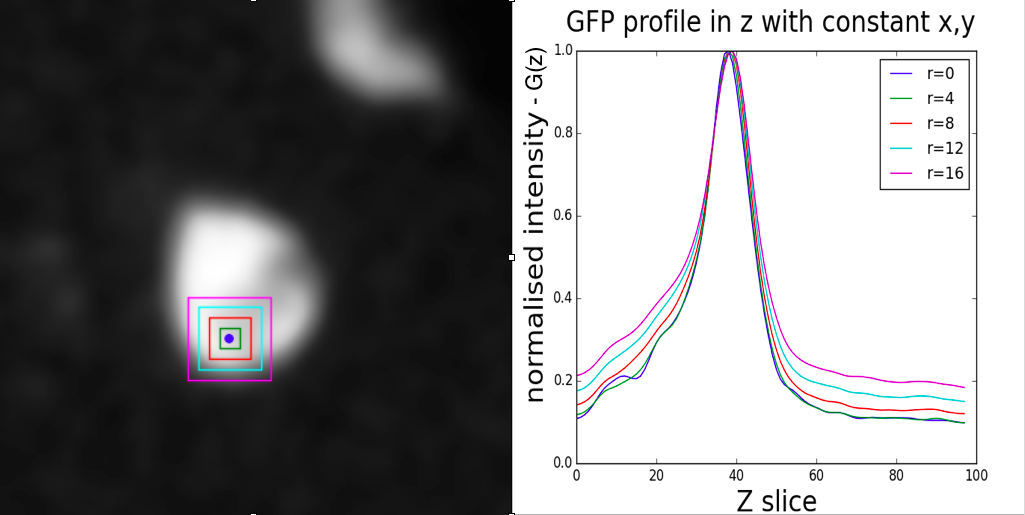
\includegraphics[width=0.9\textwidth]{401_gfp_profile}
 \caption[The GFP profile]{
 	Similar to the brightfield profile shown in Figure [ref], a profile can be generated for the GFP. This might seem to trivially be the presence of GFP at various levels since the GFP contains 3D information, where the brightfield does not. Instead, these GFP profiles can be used to interact with the brightfield, which is limited in 3D. The goal is not to segment the cell in 3D using only the GFP. In the same way as Figure [ref], three typical points show very different profiles. These can again be used in the same way to help tell the difference between different parts of the image.
 }
 \label{fig:gfpprofile}
\end{figure}

Similarly to the brightfield profile considered by Selinummi et al., measureable properties such as the variance, the location of the maximum value, and the mean value can be found for the GFP profile. The variance was found using the normalised profile, that is, the maximum value in each individual distribution is set to 1. Comparing profiles in an image can then be done using their mean value and variance. These are linearly related as shown in Figure [ref]. A background pixel will have a flat profile, giving a low variance and a high mean, since the majority of the distribution stays close the maximum value. As peaks appear in the profile due to the presence of objects, the mean will decrease, but the variance will increase proportionally. In this way, pixels with varying profile strengths can show very clearly whether they contain an object. Figure [ref] also shows a collections of blue points indicating points manually chosen to be inside cells. These are clustered in the high variance - low mean portion of the plot. The large cluster of points at low variance represent background pixels.

\begin{figure}[h!]
 \centering
 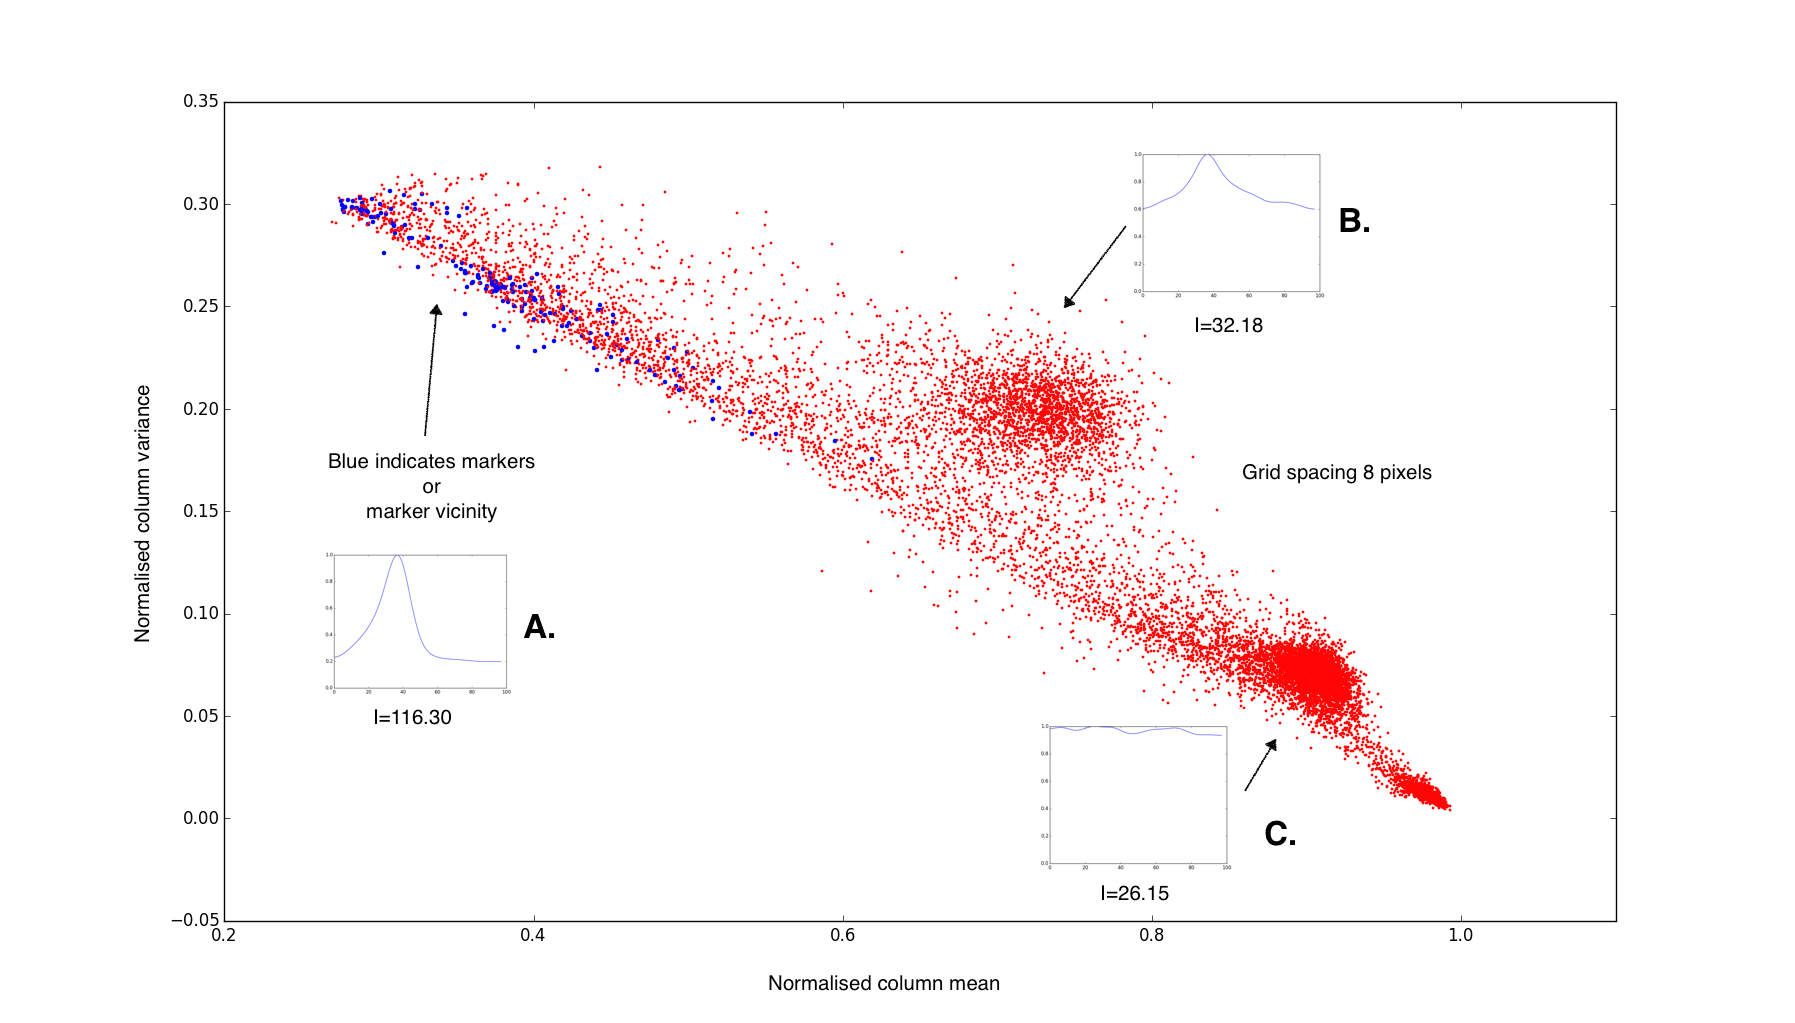
\includegraphics[width=0.9\textwidth]{402_gfp_scatter}
 \caption[GFP scatter plot]{
 	Following on from Figure [ref], different numerical properties of the profiles can be used to separate parts of the image. This plot shows a sample of points placed according to their mean and variance in intensity (not in Z). Profiles are normalised to their maximum, so a very high mean indicates a very flat distribution as in C. A very high variance, as in A, shows the presence of an object. B shows edge pixels. Each red point represents a randomly sampled point in XY. Each blue point represents a manually chosen point observed to be inside a cell in the environment. The blue points are clearly clustered towards the top left, or the high variance side of the plot. This variance will be used to later to outline cells and the provide a maximum boundary for segmentation.
 }
 \label{fig:gfpscatter}
\end{figure}

The most important part of the profile for the main method is the Z position of the maximum value. This indicates the peak intensity in the profile, and points to the most likely Z position of the part of the cell that contains the pixel in XY. This value can be used to search in the brightfield for an accurate cell representation by looking at the same level for the object in focus. Since the level indices are integers, the Z image was chosen by rounding the estimate of the Z position from the profile to the nearest integer. The more precise information is lost in the final image, but it can be stored elsewhere for further use.

\section{Optimum features for cell recognition}

By searching the brightfield with the GFP profile, the goal is to find the optimum features for segmentation. These include bright, smooth, uniformally coloured interiors surrounded by consistent, dark edges. Given a series of focal planes showing the object, it is likely that there is a single plane that contains the closest possible features to the ideal features required. This is assumed to be where the maximum GFP occurs. Unfortunately, the location of the maximum GFP for a cell shows an image that is ironically ``too focussed". When in the sharpest possible focus, a cell's edges become very thin and bright. To provide a better image for segmentation, a constant value is added to the level determined by the GFP profile. This was determined empirically and set to be between 4-8 levels added to the profile estimate. This is the second parameter for the method and is given the symbol $\Delta Z$.

For manual tracking, the accurate shape of the cell does not need to be known; it is better to see the interior of the cell clearly in order to make a good estimate of the centre to place a marker. The focal plane best for this type of observation also does not lie on plane with the maximum GFP. This shift is also empirically determined and is between 10-12 levels above the maximum GFP. This parameter is not crucial to the outcome of the method and is set by personal preference of the user tasked with finding the cells.

\section{zMod and zBF}

For each frame in time, the Z position of the maximum of the GFP profile is calculated for each pixel in XY. A new image is created, called ``zMod", where the value of each pixel proportionally represents a Z position in the environment. This is analogous to a terrain. The range of values lies between 0 and 1, but the intermediate values are discretised to multiples of $\frac{1}{numberOfZPlanes}$ in order to represent the full Z range of the experiment. Floating point representation is easier to keep track of than integer representation in an image since the float value also works as a percentage height in the environment. This map of Z positions can be smoothed to make transitions between levels more gradual. The smoothing applied used a Gaussian blur with a radius of 3 pixels. This is the third important parameter and is given the symbol $\Sigma$.

\begin{figure}[h!]
 \centering
 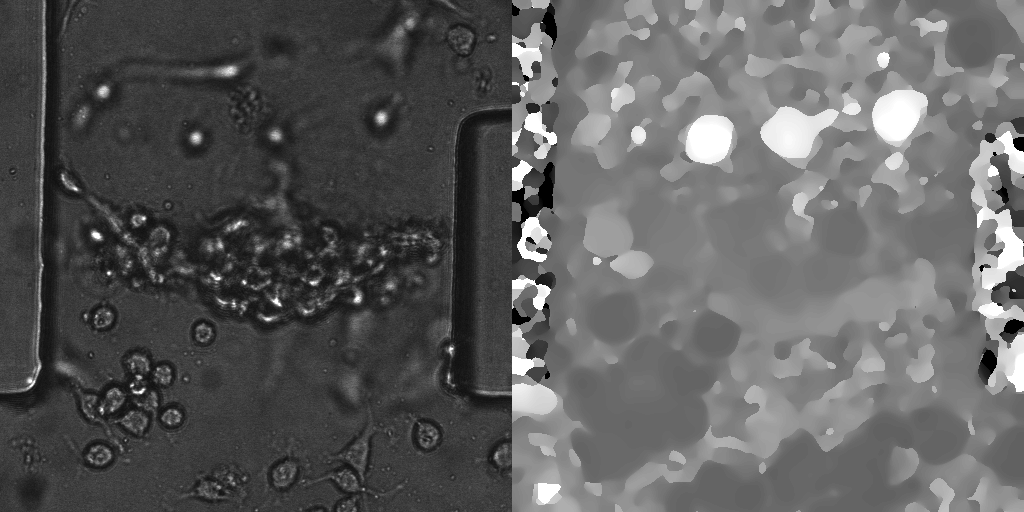
\includegraphics[width=0.9\textwidth]{403_zmod_example}
 \caption[zMod example]{
 	This is an example of the zMod result. The value of each pixel in the image is proportional to the Z value of the maximum intensity of the GFP profile. This is a rough indicator of the level of the object at this XY, but not necessarily every part of the object. In B, continuous patches of similar level correspond to cells marked with GFP. This is the second most useful result of this study as it allows information from the GFP to help find features in the brightfield.
 }
 \label{fig:zmodexample}
\end{figure}

The zMod image for each frame can be mapped to the entire set of brightfield data for the same frame by selecting a pixel value from the brightfield stack focal plane that corresponds to the Z index indiciated by the zMod image. This produces the most important result of this study, the ``zBF" image. It is a single 2D image for each frame containing representations of all objects in focus with clear edges and interiors. This works by only selecting pixel values from the levels where the objects are in focus. This does not correct the focus of objects not marked by the GFP. This image is used to segment all cells in the environment simultaneously independently of their level in the experiment using 2D segmentation techniques.

\begin{figure}[h!]
 \centering
 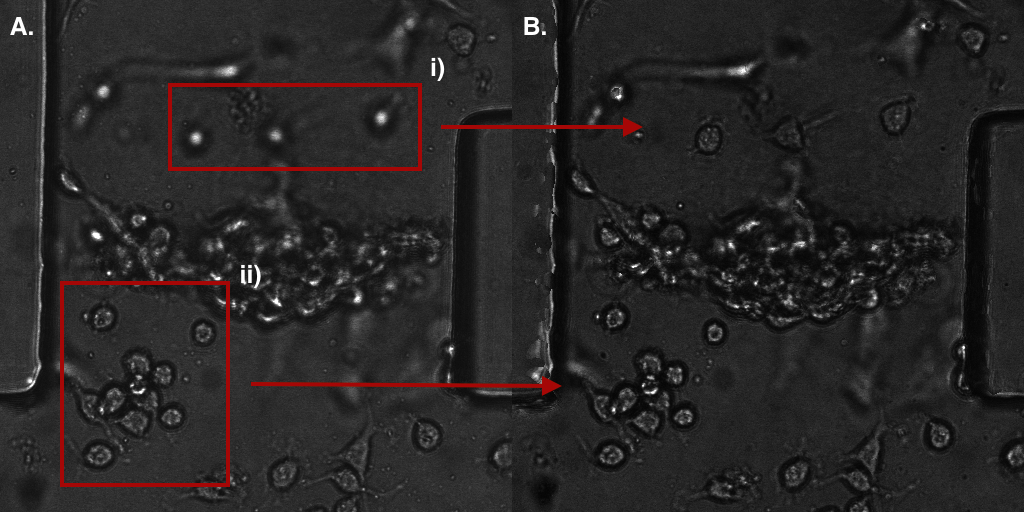
\includegraphics[width=0.9\textwidth]{404_zbf_example}
 \caption[zBF example]{
 	This image, zBF, is the most important outcome of this research. It shows that information from the GFP channel can be used to locate useful edges in the brightfield, that can in turn be used to segment cells and provide accurate numerical properties of the cells over time. It is generated by sampling from the set of brightfield data at a single frame and placing a pixel value into the final zBF image from the level indicated by zMod. In this way, the majority of the data in the brightfield stack is discarded, leaving only the most relevant information to each cell marked with GFP.
 }
 \label{fig:zbf}
\end{figure}

\section{Artificial edges for segmentation: zVar and zEdge}

A further improvement can be made to the segmentation. Part of the 3D data has already been used to correct the focus of objects marked with GFP. The part of the 3D data not used for this method is the mean (or equivalently the variance due to the linear relationship). This can indicate presence of an object more reliably than the absolute value of the GFP. Pixels with very different values in the GFP can have similar values in the mean image since the profiles are normalised such that only the shape of the distribution matters. If the mean of the normalised and inverted (since low mean/high variance indicates an object) GFP profile for each pixel in a frame is found, a new image, ``zVar" can be made. Depending on the linear smoothing of the original data (the parameter $R$), the boundary of objects in the mean image can extend beyond the edges of objects in the brightfield.

\begin{figure}[h!]
 \centering
 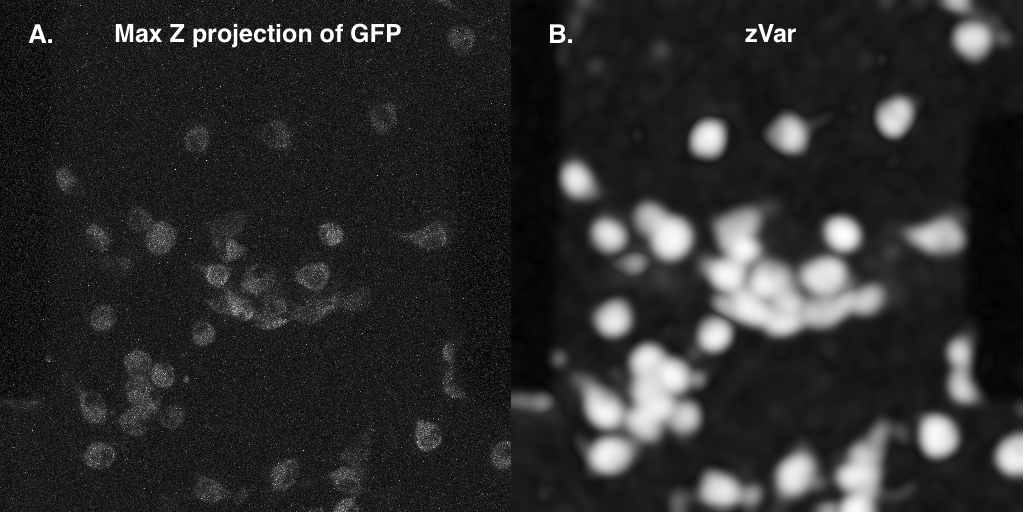
\includegraphics[width=0.9\textwidth]{405_zvar}
 \caption[zVar example]{
 	As shown in Figure [ref], each pixel in XY can be characterised by simple numerical properties such as the mean and variance of the GFP profile. Since, due to normalisation, the mean and variance are linearly dependent, one parameter can be be chosen to represent each pixel in XY. If a new image is made with this number used as the value for each pixel, the result in the zVar image. When compared with the Z-projection of the GFP, it is clear that the outlines of cells are well represented. Although the quality of the edges is not an improvement on the GFP, it shows more reliably the full extent of the cell marked by GFP. The GFP fluctuates more in different parts of the cell.
 }
 \label{fig:zvar}
\end{figure}

The extra extent of the zVar image is exploited to provide a maximum boundary for segmentation, this is combined with zMod to produce outlines around cells. This does not require the edges to be followed correctly, but only needs to enclose the general shape of the cell. These shapes are then segmented to separate objects or even rough groups of objects. The outlines of the segmentation are used to generate artificial edges using a DoF (Difference of Gaussians) edge model. These edges cut through background values that are similar in intensity to the interiors of cells. If there is a gap in the cell edge with an intensity close to the background, the segmentation will expand into the background and cause a major overestimation of the area of the cell. This image is called ``zEdge" and is the image for each frame used to provide the final segmentation data for each experiment.

\begin{figure}[h!]
 \centering
 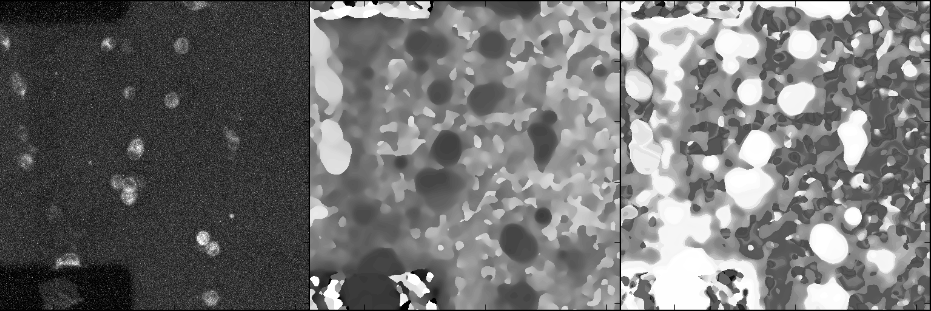
\includegraphics[width=0.9\textwidth]{406_zunique}
 \caption[zUnique example]{
 	As discussed for Figure [ref], the inconsistent amounts of the GFP intensity in different parts of the cell is compensated by looking at the variance rather than the absolute intensity. In the same way, continuous areas of similar Z can show the extent of the cell. zUnique amplifies the intensity of pixel in zVar based on the number of pixels in the image that share the same Z, in addition to being high intensity in the variance. The segmentation of this image can provide a maximum boundary for the more precise segmentation of the brightfield and prevent errors such as those shown in Figure [ref].
 }
 \label{fig:zunique}
\end{figure}

\begin{figure}[h!]
 \centering
 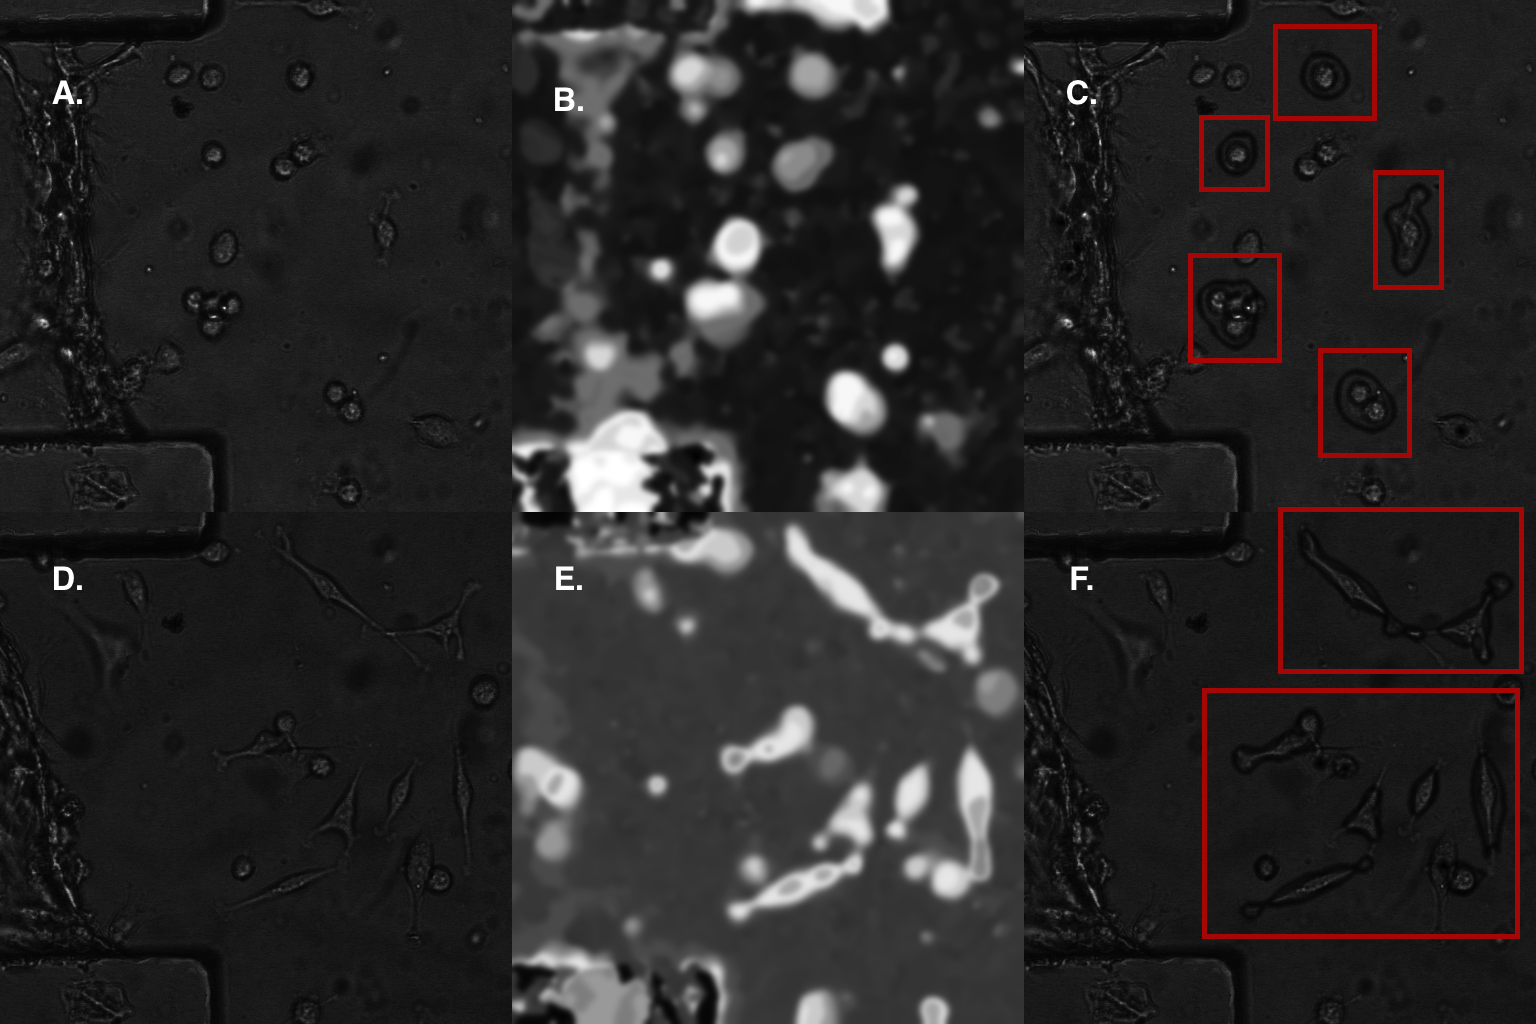
\includegraphics[width=0.9\textwidth]{407_zedge}
 \caption[zEdge example]{
 	As shown in Figure [ref], the edges in the brightfield have a particular profile. This profile in Z, and also the profile in XY, can be generalised and used to generate ``fake" edges in the image zBF image. This is done by subtracting values from the zBF according to the shape of the edge in XY. These artificial edges follow the edges of the zUnique image. This will then prevent a large amount of segmentation errors.
 }
 \label{fig:zedge}
\end{figure}

\section{Protrusion measurement}

One of the main aims of this study is to accurately measure the lengths and orientations of the cell protrusions to gather useful data on cell behaviour. The protrusions were measured by plotting the outline of the cell on a polar graph and measuring the divergence from a smooth circular shape as measured from the calculated cell centre. The protrusions show as peaks in this plot and their length is measured from the tip of the peak to the mean radius, not the centre of the cell.

\begin{figure}[h!]
 \centering
 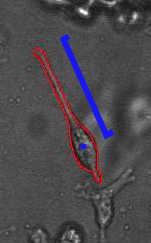
\includegraphics[width=0.3\textwidth]{408_protrusion_calculations}
 \caption[Protrusion calulation]{
 	In this study, the length of the protrusion is defined from the centre of the cell. This centre can be the manually marked point or the calculated centre of the cell mask after recognition. Both have their disadvantages. A manually chosen point might lie away from the true nucleus due to human error, but an automatically chosen point could be placed in an extension of the cell depending on the algorithm used.
 }
 \label{fig:protrusioncalc}
\end{figure}

\section{Summary of the method}

To summarise the steps taken to pre-process 3D image data for segmentation:
\begin{enumerate}
\item Smooth the data to reduce noise.
\item For each pixel in XY for the 3D data, find the vertical intensity distribution in Z, or ``profile", for each pixel nd evaluate its properties.
\item Using the profile for each pixel, create an image where the value of a pixel is proportional to the Z level of the maximum intensity of GFP at that XY location. This is zMod.
\item For zMod, there are three parameters that must be chosen: $R$, the radius of the linear smoothing kernel, which affects only the GFP in XY; $\Delta Z$, the vertical shift to locate the ideal edges for segmentation; and $\Sigma$, the size of the gaussian smoothing kernel, which affects the GFP in Z.
\item Map the Z values in zMod to the stack of image data for the brightfield. Select pixel values from the brightfield whose Z level corresponds to that indicated by zMod and place them into a new image, called zBF.
\item Although zBF now contains in-focus representations of each object marked with GFP, a further improvement can be made using the outlines of the GFP mean image. The mean image, zVar, takes the mean value of the normalised GFP profile as the value of each pixel. This gives a maximum extent of the cell and limits segmentation to a boundary to prevent it from extending into the background and incorrectly judging the area of a cell.
\item The final image, zEdge, is prepared for segmentation by using the zVar and edges of regions in zMod to automatically draw edges on the image that follow a similar edge profile to the dark edges found in the zBF image. zEdge then contains the same information as zBF, but with bounding edges beyond which the segmentation cannot extend.
\item Finally, once segmentation is complete, cell properties such as project area can be obtained along with protrusion lengths and orientations. Protrusions are found by radially plotting the distance of the edge from the centre point and designating outliers as protrusions.
\end{enumerate}

Figure [ref] below shows the full paradigm of the method.
\begin{figure}[h!]
 \centering
 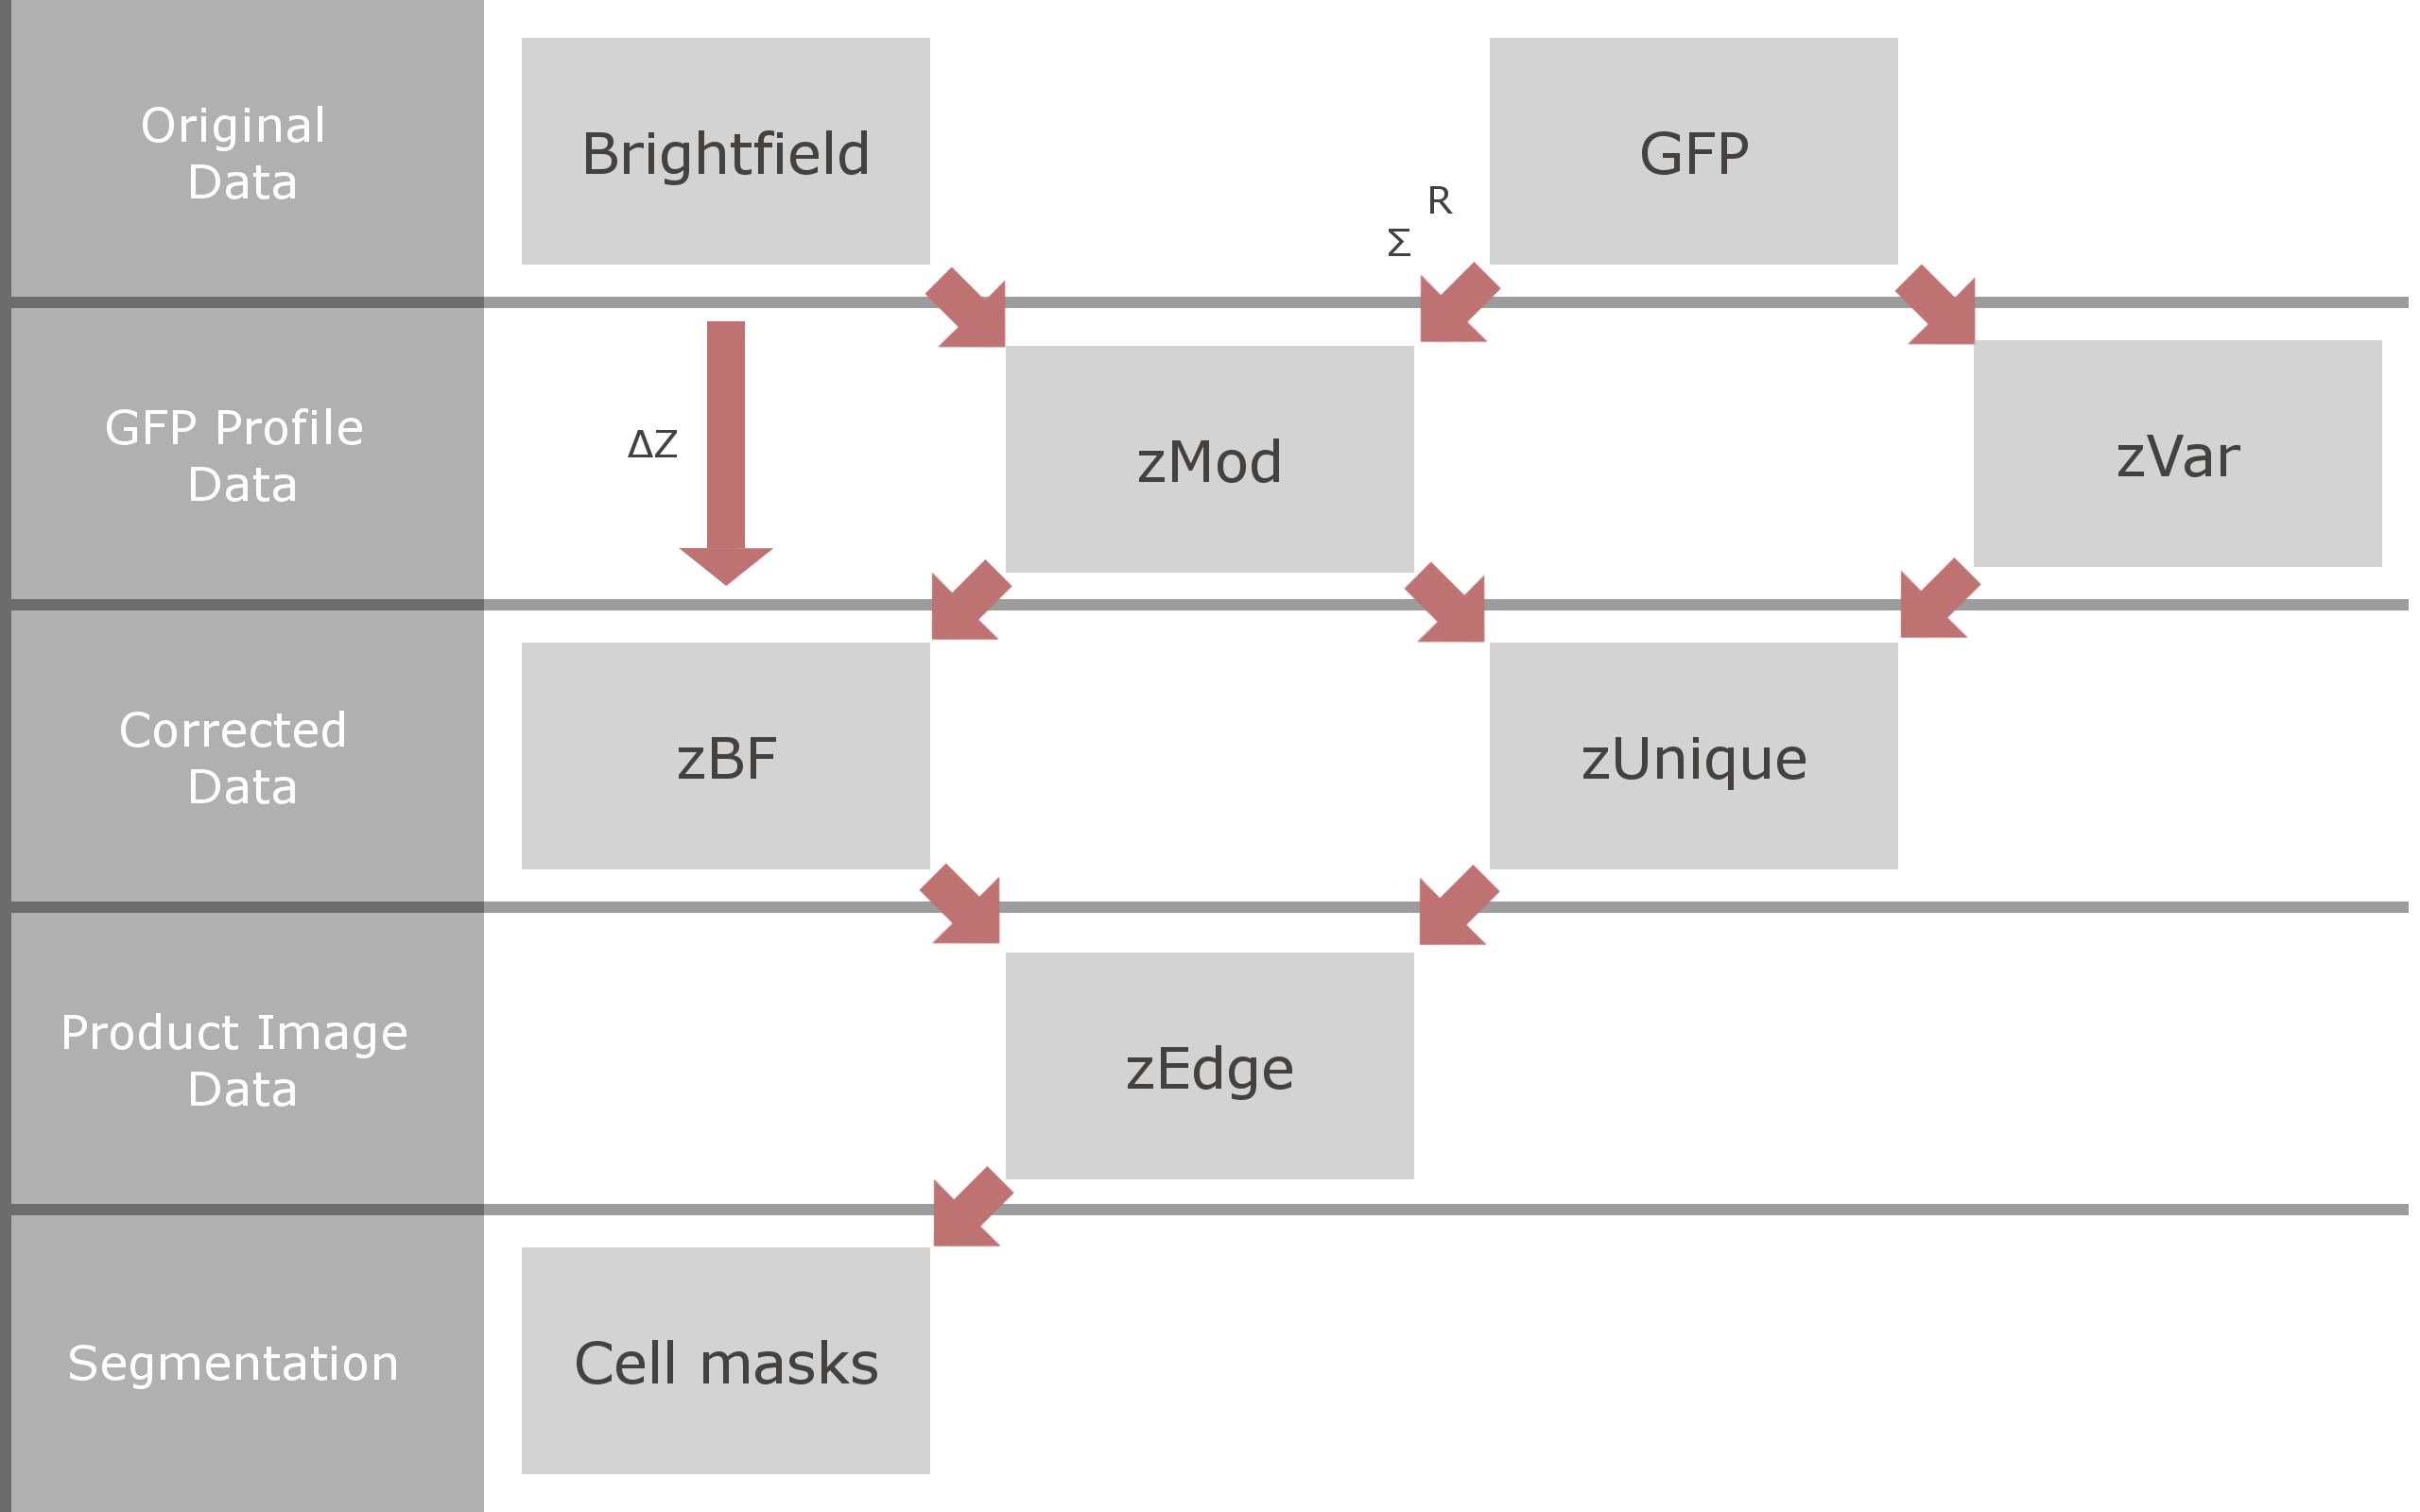
\includegraphics[width=0.9\textwidth]{409_method_flowchart}
 \caption[Method flow chart]{
 	This flow chart shows the full method from the original data to the final product images and the segmentation data. The first level shows the original data, brightfield and GFP images. They are combined along the arrows to yield products with varying uses until the final zEdge image and the segmentation are produced. Parameters used (R, $\Delta Z$, and $\Sigma$) are marked on the arrows where they are relevant.
 }
 \label{fig:flowchart}
\end{figure}

%*******************************************************************************
%****************************** Fifth Chapter *********************************
%*******************************************************************************

\chapter{Results}

\ifpdf
    \graphicspath{{Chapter5/Figs/Raster/}{Chapter5/Figs/PDF/}{Chapter5/Figs/}}
\else
    \graphicspath{{Chapter5/Figs/Vector/}{Chapter5/Figs/}}
\fi

%********************************** %First Section  **************************************
\section{Image modification}

\subsection{zMod}

%\begin{figure}[htbp!]
%\centering
%\includegraphics[width=1.0\textwidth]{}
%\caption[]{}
%\label{fig:}
%\end{figure}

%\begin{figure}[htbp!]
%\centering
%\includegraphics[width=1.0\textwidth]{}
%\caption[]{}
%\label{fig:}
%\end{figure}

\subsection{zBF}

%\begin{figure}[htbp!]
%\centering
%\includegraphics[width=1.0\textwidth]{}
%\caption[]{}
%\label{fig:}
%\end{figure}

%\begin{figure}[htbp!]
%\centering
%\includegraphics[width=1.0\textwidth]{}
%\caption[]{}
%\label{fig:}
%\end{figure}

\subsection{zEdge}

%\begin{figure}[htbp!]
%\centering
%\includegraphics[width=1.0\textwidth]{}
%\caption[]{}
%\label{fig:}
%\end{figure}

%********************************** %Second Section  **************************************
\section{Segmentation}

\subsection{GFP segmentation}

%\begin{figure}[htbp!]
%\centering
%\includegraphics[width=1.0\textwidth]{}
%\caption[]{}
%\label{fig:}
%\end{figure}

\subsection{Brightfield variance segmentation}

%\begin{figure}[htbp!]
%\centering
%\includegraphics[width=1.0\textwidth]{}
%\caption[]{}
%\label{fig:}
%\end{figure}

\subsection{zEdge segmentation}

%\begin{figure}[htbp!]
%\centering
%\includegraphics[width=1.0\textwidth]{}
%\caption[]{}
%\label{fig:}
%\end{figure}

\subsection{Manual segmentation}

%\begin{figure}[htbp!]
%\centering
%\includegraphics[width=1.0\textwidth]{}
%\caption[]{}
%\label{fig:}
%\end{figure}

%*******************************************************************************
%****************************** Fourth Chapter *********************************
%*******************************************************************************

\chapter{Results}

\ifpdf
    \graphicspath{{Chapter6/Figs/Raster/}{Chapter6/Figs/PDF/}{Chapter6/Figs/}}
\else
    \graphicspath{{Chapter6/Figs/Vector/}{Chapter6/Figs/}}
\fi

%********************************** %First Section  **************************************
\section{Image modification}

\subsection{zMod}

\begin{figure}[htbp!]
\centering
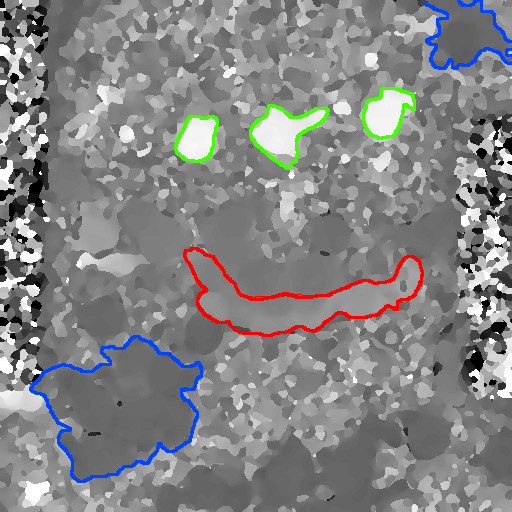
\includegraphics[width=1.0\textwidth]{5111-zmod_example_outline-050714_s13_ch-zmod-8-3-3_t0_z00}
\caption[zMod example]{An example of the zMod result.}
\label{fig:zmod_result}
\end{figure}

Although the cell outlines are not clearly visible, regions that contain cells have very uniform z-locations. Even regions outside the cells have assigned z-locations; this includes background noise and the even lower levels of background noise found in the PDMS pillars. An example is shown in Figure~\ref{fig:zmod_result}. Groups of cells at a low level are outlined in blue, mid level cells adjacent to the barrier in red, and high level cells in green.

It should be noted that this image does not indicate anything about the absolute intensity of the GFP or the Brightfield.

It is clear that there are two types of background noise: the environment and the PDMS pillars. The zMod values inside the pillars are more highly variable.

Regions of similar level are quite contiguous, even in the background. This indicates a certain amount of smoothing of the GFP (R=3, $\Sigma$=3). Smoothing was done with a Gaussian filter. The smoothing also causes the gradual transitions between adjacent regions of similar levels.

The three bright blobs at the top of the image represent three cells that lie at a high z-level in the image. At the bottom of the image, the very dark regions indicate a collection of cells that lie very low in the z-dimension of the 3D environment. It should be noted that some cells in the barrier have higher intensity than the cells below the barrier. There is a ring of lighter cancer cells in the middle. They are attached to the barrier.

This image does not indicate whether any cells overlap. It also does not reveal detailed protrusions or clear boundaries of individual cells.

\begin{figure}[htbp!]
\centering
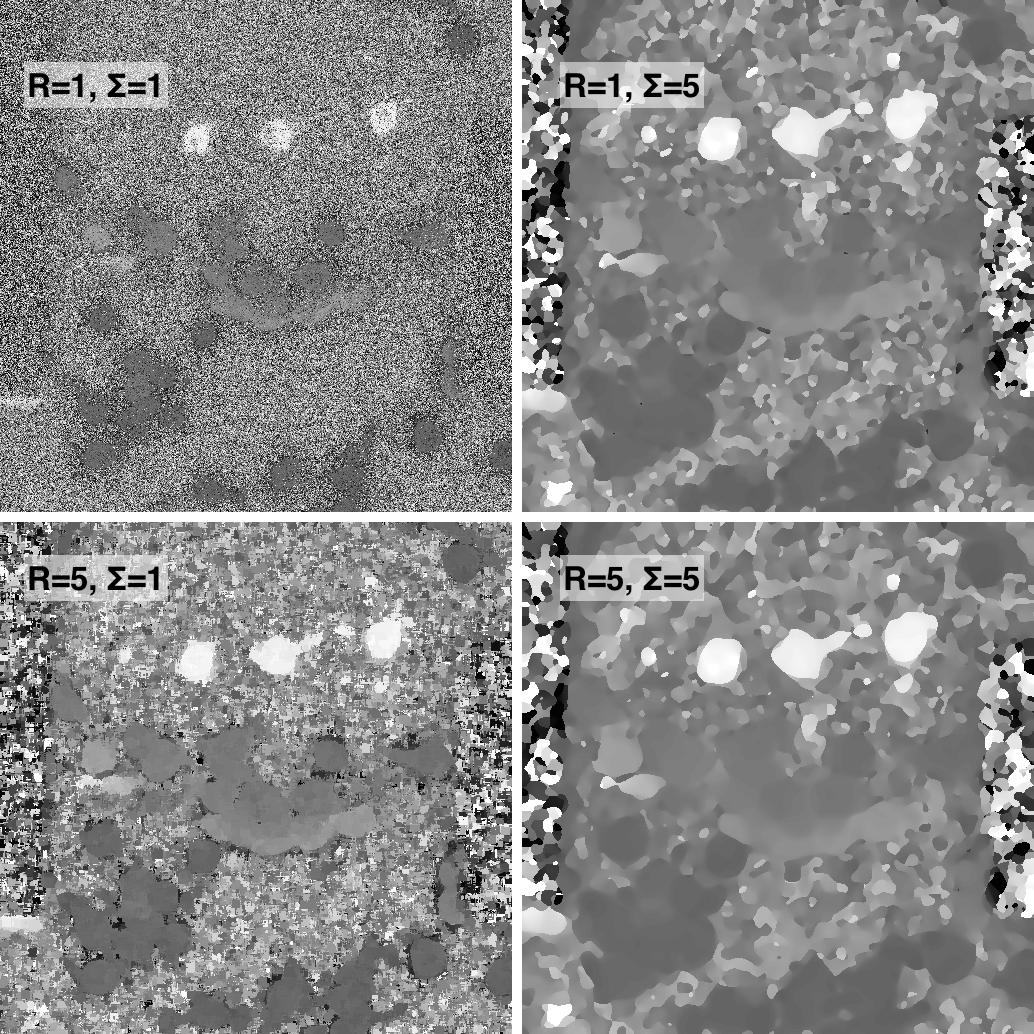
\includegraphics[width=1.0\textwidth]{5-combined_R_sigma}
\caption{The extremes of R and $\Sigma$}
\label{fig:r_and_sigma}
\end{figure}

The two main parameters that we can vary are R and $\Sigma$. The maximum values and their results are shown in Figure~\ref{fig:r_and_sigma}.

R indicates the size of the mask used to search around the x-y position of a pixel for GFP information to use in estimating the z-position of that pixel. If R=1, only information immediately in that pixel is used to make that decision and thus the z-levels of neighbouring GFP profiles do not affect each other.

If R=5, an 11-by-11 square of pixels profiles centred on the x-y position produces the final estimate of z. This can lead to larger contiguous regions sharing similar z-values. It is worth noting that smoothing or "mixing" of z-levels occurs in 3D. Since information from every profile inside the mask is taken into account, intensities at all levels will contribute to the estimate of the z-value.

$\Sigma$ is the size of the Gaussian kernel used to smooth the GFP in 2D. The smoothing is performed before GFP profiles are generated and analysed. Since the smoothing is performed in 2D, cells that exist at very different levels in z but close proximity in x-y will not affect the profiles in each other's pixels during smoothing. If $\Sigma$=1, little smoothing is performed and the image is very noisy. The z-levels of the pixels inside the cells are less uniform. The cells are grainy. If R=5 and $\Sigma$=1, an effect similar to aliasing is visible [ref]. This is because of the discrete size of the mask set by R. It still appears noisy, but the effects of the noise have been spread out and diminished.

As R increases, the continuous area of the cell becomes more uniform. It is however still noisy. As $\Sigma$ increases, the effect of noise is diminished. This is because increasing R does not decrease the noise, it simply distributes its effects more widely within a mask, which has an averaging effect on a cell interior. On the other hand, increasing $\Sigma$ does actually reduce the absolute level of noise.

If $\Sigma$=1, then the transitions between z-levels are sharper. The noise in the GFP will have a larger effect on the selection of the z-level if the GFP is not smoothed. If $\Sigma$=5, then there is a large amount of smoothing, and noise is greatly reduced, producing more gentler transitions between parts of the same cell.

\subsection{zBF}

\begin{figure}[htbp!]
\centering
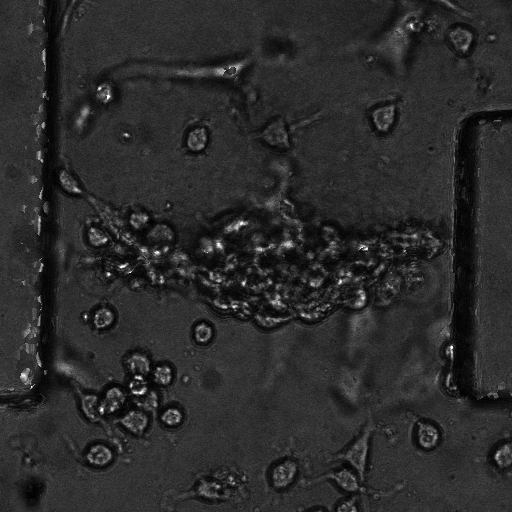
\includegraphics[width=1.0\textwidth]{5121-zbf_example-050714_s13_ch-zbf-8-3-3_t0_z00}
\caption{An example of zBF.}
\label{fig:zbf_example}
\end{figure}

As seen in Figure~\ref{fig:zbf_example}, all cells previously marked with GFP are now in focus, regardless of their z-level in the 3D environment. Delta-z has been adjusted manually to optimise the features of the cells for segmentation, i.e. where the Brightfield edges are as dark as possible and the Brightfield cell interiors are as uniform as possible. If delta-z were chosen to be higher or lower, the entire environment would appear slightly out of focus. The interiors of the cells are often non-uniform but have a higher intensity than the background. Some protrusions can clearly be seen, but others have been hidden or appear closer to the intensity of the background because they did not contain enough GFP to be adjusted by zMod properly.

The intensities in the background (notably the pillars) are highly randomised. This is due to the highly random nature of zMod in these regions but it does not directly affect the segmentation of the cancer cells.

There are some cells that appear out-of-focus such as within, above, and below the barrier. This is because they were not initially marked with GFP, so the z-position that zMod assigns to them is fairly arbitrary. The intensity profiles of these pixels are very flat, so even a small variation due to noise will cause a maximum in z to be located randomly.

\subsection{zEdge}

\begin{figure}[htbp!]
\centering
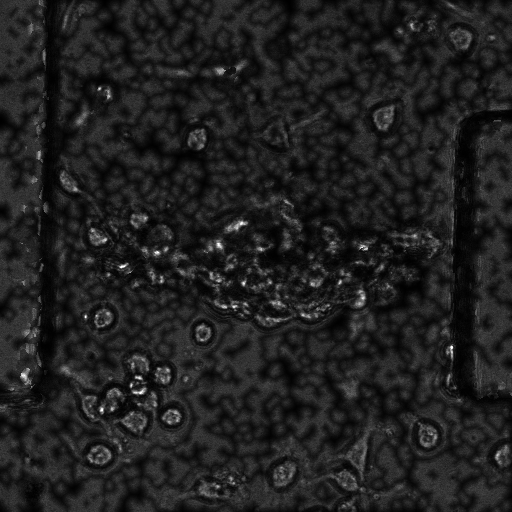
\includegraphics[width=1.0\textwidth]{5122-zedge_example-050714_s13_ch-zedge-8-3-3_t0_z00}
\caption{An example of zEdge}
\label{fig:zedge_example}
\end{figure}

The edges drawn on zEdge are similar to the Brightfield cell boundaries but are more distinct and regular, shown in Figure~\ref{fig:zedge_example}. These edges closely approximate the true boundaries of the cells. They are also better defined, which will prevent the segmentation from spilling over into the background. The edges drawn in the background are highly randomised, but this will have no effect on segmentation because there are no markers in the background.

%********************************** %Second Section  **************************************
\section{Segmentation}

\subsection{Segmentation results}

\begin{figure}[htbp!]
\centering
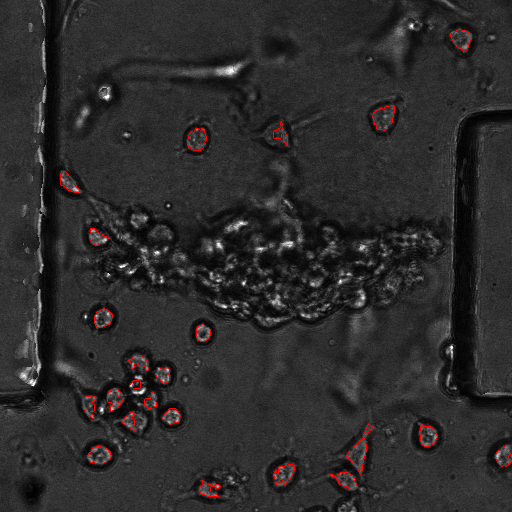
\includegraphics[width=1.0\textwidth]{5224-zedge_seg-tile_050714_s13_ch-zbf-8-5-5-outline-zcomp-8-1-1-zedge-8-5-5-TYOGE5XI_t0}
\caption{zEdge segmentation}
\label{fig:zedge_segmentation}
\end{figure}

Most of the segmentation results, shown in Figure~\ref{fig:zedge_segmentation}, very closely match the dark edges of the Brightfield. Some of the segmentation fails, especially when the interior of the cell is very non-uniform. In the bottom left of Figure~\ref{fig:zedge_segmentation}, there is a cluster of cells, in which there is a cell at the centre of this cluster for which segmentation has failed. The protrusions are not very well recognised, either because zEdge is limiting the protrusions or the protrusions are not distinct enough from the background because of the lack of GFP within them.

\begin{figure}[htbp!]
\centering
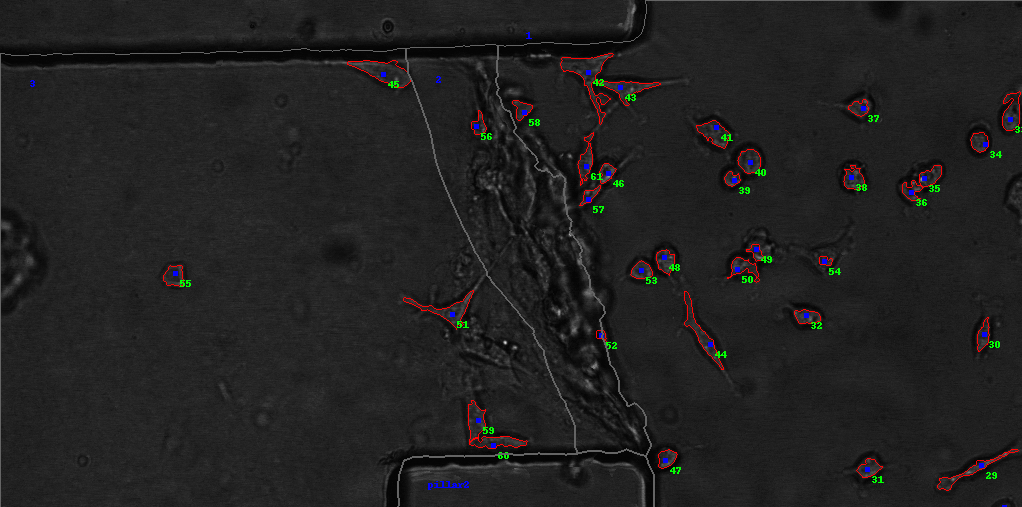
\includegraphics[width=1.0\textwidth]{good_protrusions-tile_260714_s14_t016}
\caption{Accurately segmented protrusions using zEdge.}
\label{fig:accurate_zedge}
\end{figure}

Figure~\ref{fig:accurate_zedge}, taken from another experiment from which we gathered data, is included for illustrative purposes. In this series, the cell protrusions contain more GFP and extend further from the cells. This image showcases the results of applying the zMod method more clearly in terms of protrusions. Particularly noteworthy are Cells 43, 44, and 51, whose recognitions extend very far into their protrusions with no spillover effects. Admittedly, the protrusions are still longer than the segmentation results, due to the boundaries imposed by zEdge.

\subsection{Fscore comparison}

\subsubsection{Manual ground truth}

\begin{figure}[htbp!]
\centering
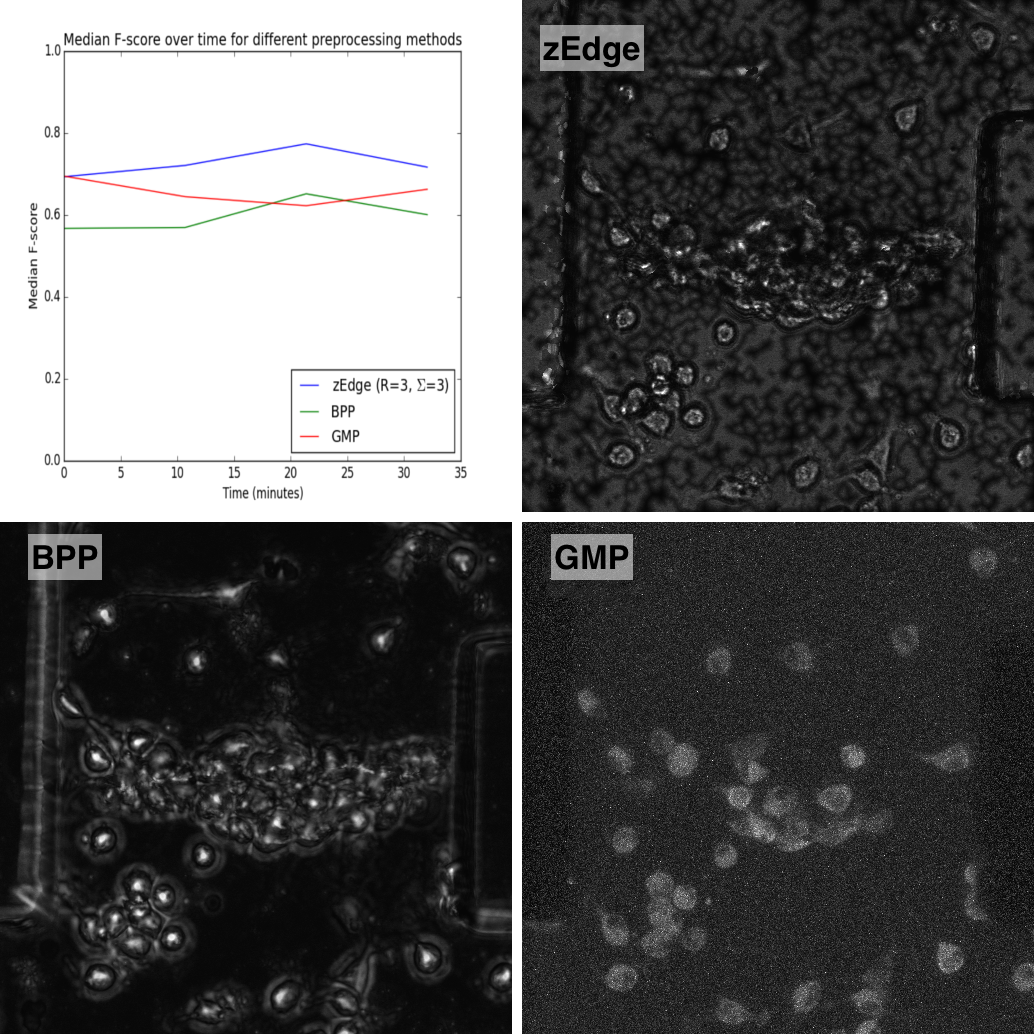
\includegraphics[width=1.0\textwidth]{6211-fscore_manual-GT_zmod_r3_s3-gmod-bmod}
\caption{Manual ground truth results}
\label{fig:manual_ground}
\end{figure}

In Figure~\ref{fig:manual_ground}, we take the result of manual segmentation to be the ground truth. The line labelled zMod represents the results of the method we propose. The line labelled bMod represents the results of the method used by Selinummi et al. The line labelled gMod represents the result of the segmentation of the GFP maximum, in which the maximum of each 3D profile in z is selected as the value for that 2D x-y position. gMod is used as ground truth in the paper by Selinummi et al.

All three of the Fscore values over time stay quite consistent. zMod has a greater median value than that of either gMod (Selinummi's ground truth) or bMod (their test method).

\subsubsection{Fluorescence ground truth}

\begin{figure}[htbp!]
\centering
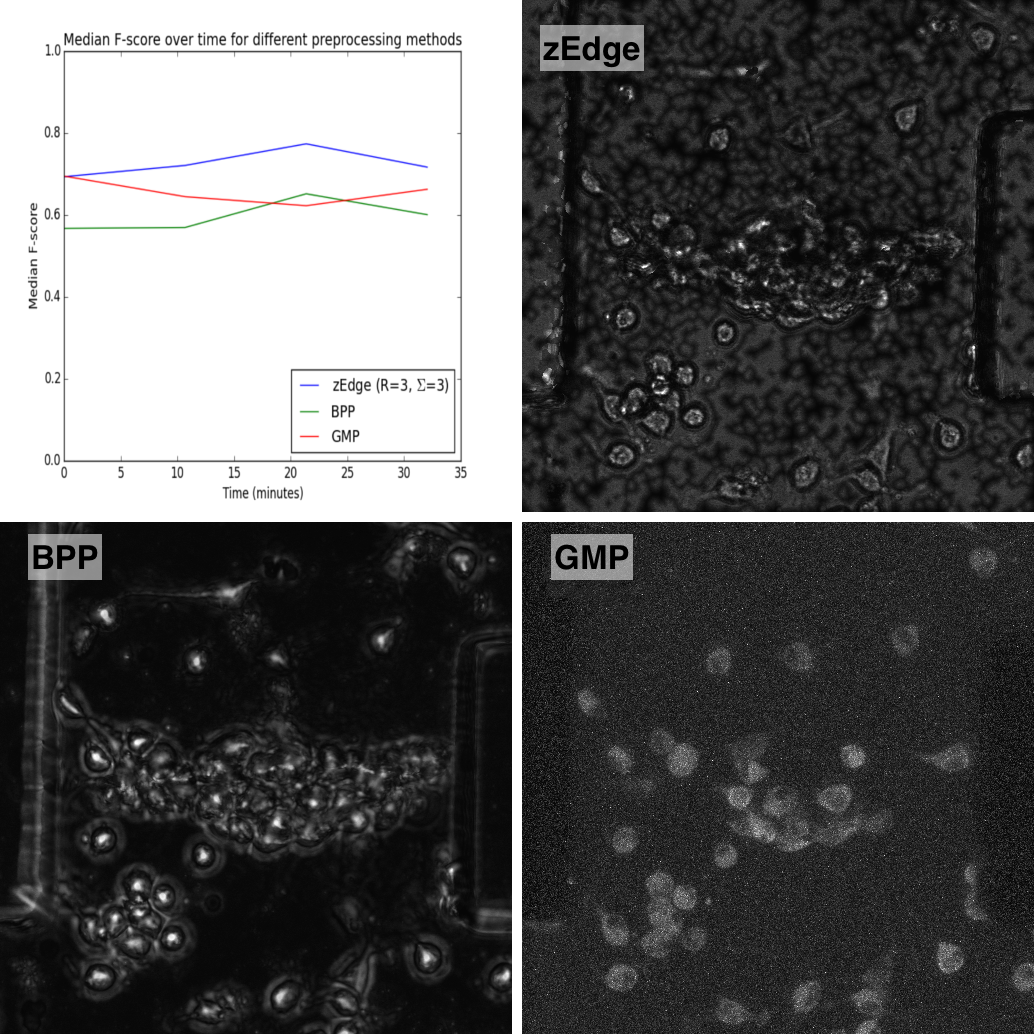
\includegraphics[width=1.0\textwidth]{6211-fscore_manual-GT_zmod_r3_s3-gmod-bmod}
\caption{GFP maximum projection segmentation}
\label{fig:gfp_maximum}
\end{figure}

In Figure~\ref{fig:gfp_maximum}, both of the methods zMod and bMod, with reference to maximum fluorescence levels used as ground truth (as seen in the Selinummi paper), have very constant median Fscores. The zMod Fscore is above the bMod Fscore.

\subsection{zMod sensitivity analysis}

\begin{figure}[htbp!]
\centering
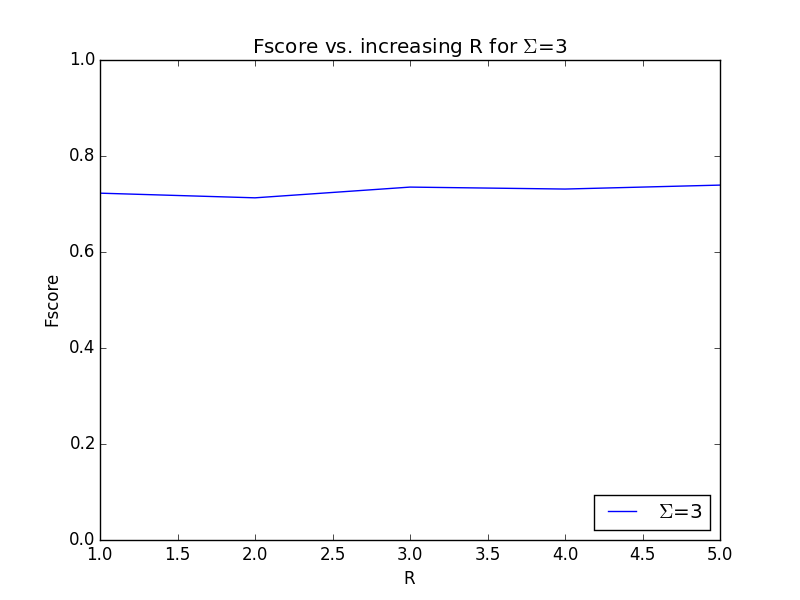
\includegraphics[width=1.0\textwidth]{6213-fscore_R_for_sigma3}
\caption{Fscore results for increasing R at constant $\Sigma=3$}
\label{fig:fscore_sigma3}
\end{figure}

The Fscore for our method, zMod, does not vary significantly with increasing R, as shown in Figure~\ref{fig:fscore_sigma3}. This means that the quality of the segmentation, using standard values for segmentation parameters, is independent of the R-value or the size of the mask linearly mixing the z-values. This would not necessarily be the case with large numbers of cells that overlapped in the z-dimension.

\begin{figure}[htbp!]
\centering
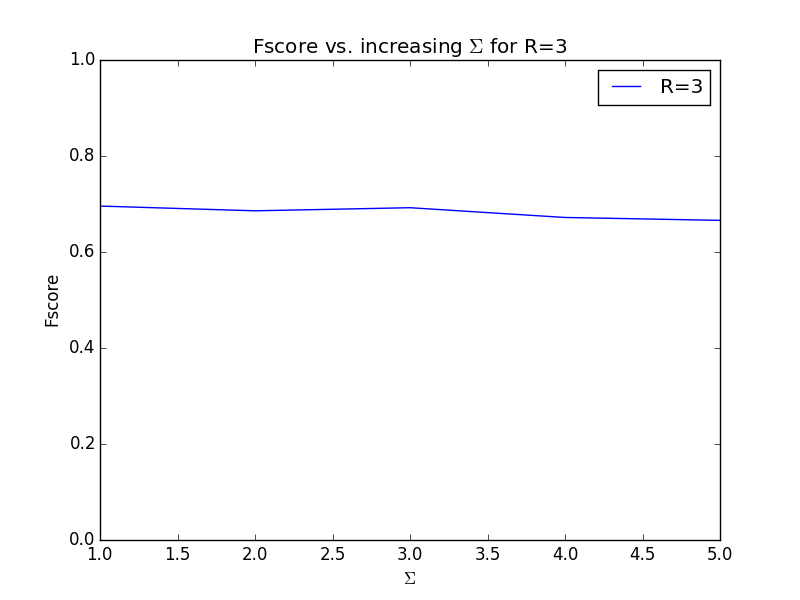
\includegraphics[width=1.0\textwidth]{6222-fscore_sigma_for_R3}
\caption{Fscore results for increasing $\Sigma$ at constant $R=3$}
\label{fig:fscore_r3}
\end{figure}

Holding R constant, the Fscore does not vary significantly with increasing $\Sigma$, as shown in Figure~\ref{fig:fscore_r3}. This indicates that the smoothing of the GFP in 2D has little effect on zMod and, in turn, on zEdge.

%*******************************************************************************
%****************************** Fourth Chapter *********************************
%*******************************************************************************

\chapter{Discussion}

\ifpdf
    \graphicspath{{Chapter7/Figs/Raster/}{Chapter7/Figs/PDF/}{Chapter7/Figs/}}
\else
    \graphicspath{{Chapter7/Figs/Vector/}{Chapter7/Figs/}}
\fi

\section{zEdge segmentation results}

\begin{figure}[htbp!]
\centering
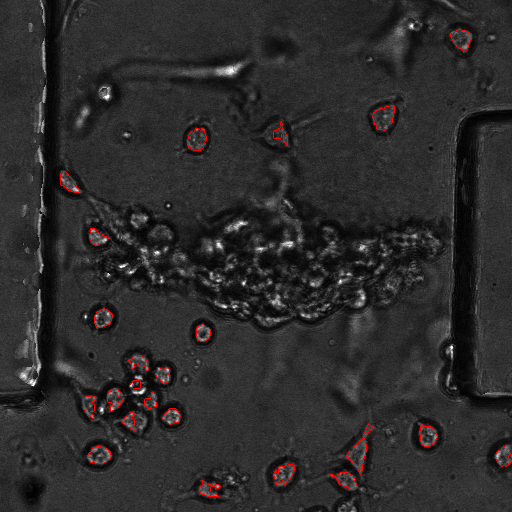
\includegraphics[width=1.0\textwidth]{5224-zedge_seg-tile_050714_s13_ch-zbf-8-5-5-outline-zcomp-8-1-1-zedge-8-5-5-TYOGE5XI_t0}
\caption{zEdge segmentation}
\label{fig:zedge_segmentation}
\end{figure}

Several cells in Figure~\ref{fig:zedge_segmentation} were mis-recognised. The cell in the centre of the group on the lower left is a good example. The mis-recognition in this case is due to bright flecks in the interior of the cell that prevent the segmentation from extending from the marker to other locations in the interior. This could be ameliorated by selectively smoothing the brightfield inside the edges. Unfortunately, this process would also dampen the appearance of other parts of the cells, such as protrusions, that have poorly defined edges. An analogous situation occurs in GFP images [ref Arce].

Another mis-recognition occurs in the cell at the top of the image in the centre of the group of three. This does not appear to be a result of highly non-uniform interior, but the segmentation algorithm did not allow the recognition to continue. This can be improved by increasing the contrast between the cell interior and the background, causing the cell interior to appear to be of higher value than the background and allowing the segmentation to continue.

In general, mis-recognition occurs when there is no clear reason for the segmentation to continue. This is also dependent on the starting location of the marker in the Brightfield. Another starting location with a higher intensity will be more likely to fill the lower intensities around it.

\section{zMod sensitivity results}

We expected that the correspondence between the manual segmentation ground truth and the zEdge segmentation would increase when the noise was reduced (by increasing Sigma). Increasing R (the size of the mask used to produce the GFP pixel profile for each x-y position) was expected to mix the z-levels in neighbouring pixels to make contiguous regions of similar z-levels more uniform. This was observed in the resulting images.

However, neither increased R nor increased Sigma had significant effect on the Fscore of our preprocessed images. We had thought that smoother, less noisy images would produce more accurate segmentation, but this is contradicted by the Fscore results. The method itself, however, still yields higher Fscores than the method described by Selinummi et al.

\section{Comparison of preprocessing methods}

\begin{figure}[htbp!]
\centering
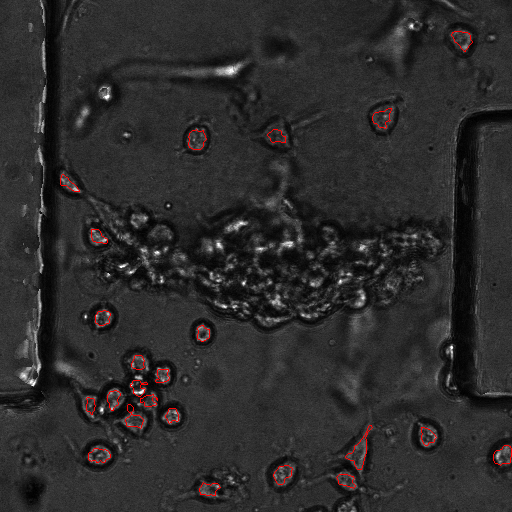
\includegraphics[width=1.0\textwidth]{5223-bf_std_seg-tile_050714_s13_ch-zbf-8-5-5-outline-zcomp-8-1-1-bmod-PLG5WADE_t0}
\caption{bMod segmentation}
\label{fig:bmod_segmentation}
\end{figure}

Both segmentation results in Figure~\ref{fig:bmod_segmentation} do fairly well at picking up the general shape of the cells.

Our segmentation more consistently approximates the dark Brightfield edges. It appears as though the Selinummi method compresses the segmentation; its resulting edges lie away from the true edges. It instead produces edges that are closer to the interior of the cell. This probably explains the decrease in Fscore for this method.

The regions assigned a higher contrast by the Selinummi method have highly variable Brightfield profiles in the z-dimension. In the Brightfield data, the locations of the true edges will not have highly variable profiles. Instead, the regions immediately on either side of the edge will be the most highly variable, as these are where Brightfield intensity discontinuities actually occur. The Selinummi method looks for this disturbances in order to find cell edge pixels. This causes a systematic underestimation of the extent of the cell. In contrast, our method use GFP intensity pixel profiles to select an image section from the Brightfield stack for each cell pixel or group of cell pixels. We thus preserve the darker edges and strengthen them.

%*******************************************************************************
%****************************** Fourth Chapter *********************************
%*******************************************************************************

\chapter{}

\ifpdf
    \graphicspath{{Chapter8/Figs/Raster/}{Chapter8/Figs/PDF/}{Chapter8/Figs/}}
\else
    \graphicspath{{Chapter8/Figs/Vector/}{Chapter8/Figs/}}
\fi

%********************************** %First Section  **************************************


% ********************************** Back Matter *******************************
% Backmatter should be commented out, if you are using appendices after References
%\backmatter

% ********************************** Bibliography ******************************
\begin{spacing}{0.9}

% To use the conventional natbib style referencing
% Bibliography style previews: http://nodonn.tipido.net/bibstyle.php
% Reference styles: http://sites.stat.psu.edu/~surajit/present/bib.htm

\bibliographystyle{apalike}
%\bibliographystyle{unsrt} % Use for unsorted references
%\bibliographystyle{plainnat} % use this to have URLs listed in References
\cleardoublepage
\bibliography{References/references} % Path to your References.bib file


% If you would like to use BibLaTeX for your references, pass `custombib' as
% an option in the document class. The location of 'reference.bib' should be
% specified in the preamble.tex file in the custombib section.
% Comment out the lines related to natbib above and uncomment the following line.

%\printbibliography[heading=bibintoc, title={References}]


\end{spacing}

% ********************************** Appendices ********************************

\begin{appendices} % Using appendices environment for more functunality

% ******************************* Thesis Appendix A ****************************
\chapter{How to install \LaTeX} 

\section*{Windows OS}

\subsection*{TeXLive package - full version}
\begin{enumerate}
\item	Download the TeXLive ISO (2.2GB) from\\
\href{https://www.tug.org/texlive/}{https://www.tug.org/texlive/}
\item	Download WinCDEmu (if you don't have a virtual drive) from \\
\href{http://wincdemu.sysprogs.org/download/}
{http://wincdemu.sysprogs.org/download/}
\item	To install Windows CD Emulator follow the instructions at\\
\href{http://wincdemu.sysprogs.org/tutorials/install/}
{http://wincdemu.sysprogs.org/tutorials/install/}
\item	Right click the iso and mount it using the WinCDEmu as shown in \\
\href{http://wincdemu.sysprogs.org/tutorials/mount/}{
http://wincdemu.sysprogs.org/tutorials/mount/}
\item	Open your virtual drive and run setup.pl
\end{enumerate}

or

\subsection*{Basic MikTeX - \TeX~ distribution}
\begin{enumerate}
\item	Download Basic-MiK\TeX (32bit or 64bit) from\\
\href{http://miktex.org/download}{http://miktex.org/download}
\item	Run the installer 
\item	To add a new package go to Start >> All Programs >> MikTex >> Maintenance (Admin) and choose Package Manager
\item	Select or search for packages to install
\end{enumerate}

\subsection*{TexStudio - \TeX~ editor}
\begin{enumerate}
\item	Download TexStudio from\\
\href{http://texstudio.sourceforge.net/\#downloads}
{http://texstudio.sourceforge.net/\#downloads} 
\item	Run the installer
\end{enumerate}

\section*{Mac OS X}
\subsection*{MacTeX - \TeX~ distribution}
\begin{enumerate}
\item	Download the file from\\
\href{https://www.tug.org/mactex/}{https://www.tug.org/mactex/}
\item	Extract and double click to run the installer. It does the entire configuration, sit back and relax.
\end{enumerate}

\subsection*{TexStudio - \TeX~ editor}
\begin{enumerate}
\item	Download TexStudio from\\
\href{http://texstudio.sourceforge.net/\#downloads}
{http://texstudio.sourceforge.net/\#downloads} 
\item	Extract and Start
\end{enumerate}


\section*{Unix/Linux}
\subsection*{TeXLive - \TeX~ distribution}
\subsubsection*{Getting the distribution:}
\begin{enumerate}
\item	TexLive can be downloaded from\\
\href{http://www.tug.org/texlive/acquire-netinstall.html}
{http://www.tug.org/texlive/acquire-netinstall.html}.
\item	TexLive is provided by most operating system you can use (rpm,apt-get or yum) to get TexLive distributions
\end{enumerate}

\subsubsection*{Installation}
\begin{enumerate}
\item	Mount the ISO file in the mnt directory
\begin{verbatim}
mount -t iso9660 -o ro,loop,noauto /your/texlive####.iso /mnt
\end{verbatim}

\item	Install wget on your OS (use rpm, apt-get or yum install)
\item	Run the installer script install-tl.
\begin{verbatim}
	cd /your/download/directory
	./install-tl
\end{verbatim}
\item	Enter command `i' for installation

\item	Post-Installation configuration:\\
\href{http://www.tug.org/texlive/doc/texlive-en/texlive-en.html\#x1-320003.4.1}
{http://www.tug.org/texlive/doc/texlive-en/texlive-en.html\#x1-320003.4.1} 
\item	Set the path for the directory of TexLive binaries in your .bashrc file
\end{enumerate}

\subsubsection*{For 32bit OS}
For Bourne-compatible shells such as bash, and using Intel x86 GNU/Linux and a default directory setup as an example, the file to edit might be \begin{verbatim}
edit $~/.bashrc file and add following lines
PATH=/usr/local/texlive/2011/bin/i386-linux:$PATH; 
export PATH 
MANPATH=/usr/local/texlive/2011/texmf/doc/man:$MANPATH;
export MANPATH 
INFOPATH=/usr/local/texlive/2011/texmf/doc/info:$INFOPATH;
export INFOPATH
\end{verbatim}
\subsubsection*{For 64bit OS}
\begin{verbatim}
edit $~/.bashrc file and add following lines
PATH=/usr/local/texlive/2011/bin/x86_64-linux:$PATH;
export PATH 
MANPATH=/usr/local/texlive/2011/texmf/doc/man:$MANPATH;
export MANPATH 
INFOPATH=/usr/local/texlive/2011/texmf/doc/info:$INFOPATH;
export INFOPATH

\end{verbatim}



%\subsection{Installing directly using Linux packages} 
\subsubsection*{Fedora/RedHat/CentOS:}
\begin{verbatim} 
sudo yum install texlive 
sudo yum install psutils 
\end{verbatim}


\subsubsection*{SUSE:}
\begin{verbatim}
sudo zypper install texlive
\end{verbatim}


\subsubsection*{Debian/Ubuntu:}
\begin{verbatim} 
sudo apt-get install texlive texlive-latex-extra 
sudo apt-get install psutils
\end{verbatim}

% ******************************* Thesis Appendix B ********************************

\chapter{Installing the CUED class file}

\LaTeX.cls files can be accessed system-wide when they are placed in the
<texmf>/tex/latex directory, where <texmf> is the root directory of the user’s \TeX installation. On systems that have a local texmf tree (<texmflocal>), which
may be named ``texmf-local'' or ``localtexmf'', it may be advisable to install packages in <texmflocal>, rather than <texmf> as the contents of the former, unlike that of the latter, are preserved after the \LaTeX system is reinstalled and/or upgraded.

It is recommended that the user create a subdirectory <texmf>/tex/latex/CUED for all CUED related \LaTeX class and package files. On some \LaTeX systems, the directory look-up tables will need to be refreshed after making additions or deletions to the system files. For \TeX Live systems this is accomplished via executing ``texhash'' as root. MIK\TeX users can run ``initexmf -u'' to accomplish the same thing.

Users not willing or able to install the files system-wide can install them in their personal directories, but will then have to provide the path (full or relative) in addition to the filename when referring to them in \LaTeX.

\end{appendices}

% *************************************** Index ********************************
\printthesisindex % If index is present

\end{document}
